% !TEX root = thesis.tex
\chapter{Complex of Strongly Separating Curves}
\label{chap:strongsep}

The content of this chapter is joint work with Alan McLeay at the University of Glasgow.

The complex of strongly separating spheres $\mathcal C^{ss}S_{g,p} \subset \mathcal C S_{g,p}$ is the induced subcomplex
whose vertices are
separating curves in the genus $g$, $n$-punctured surface $S_{g,p}$
such that both components have complexity $3g'+p'-3 > 0$.
In particular
$$
\css S_{g,p} = \csep S_{g,p}
$$
is the complex of separatng curves whenever $p \leq 1$,
and otherwise $
\css S_{g,p} \subset \csep S_{g,p}
$
is the subcomplex discarding curves bounding pairs of pants.

In
\cite{MR3724237,MR3620458}
Bowditch demonstrates that if $\aaut \css S_{g,p}$ is the mapping class group,
then
 every quasi-isometry of the
Weil-Petersson metric on Teichm\"uller space associated to $S_{g,p}$
is induced by a mapping class of $S_{g,p}$.
In \cite{bowditch} Bowditch completes the reduction by showing that
$\aaut \css S_{g,p}$ is the mapping class group in all but finitely many cases.


\begin{theorem}
  \label{thm:bowditch}
 If $g+p\geq 7$, then
 the natural map
 $$\mcg^\pm \left ( S_{g,p} \right ) \to \aaut \left ( C^{ss}(S_{g,p}) \right )$$
 is an isomorphism.
\end{theorem}

Bowditch asks which of the remaining low complexity $g+p \leq 6$ cases have $\aaut \css S_{g,p}$ given by the mapping class group.
In this chapter we provide an independent proof of Bowditch's result that settles some of these low complexity cases and
 provide evidence that the remaining unknown cases of $\aaut \css$ are themselves mapping class groups.
The goal of this chapter is to prove the following theorem.

\begin{theorem}
  \label{thm:css}
The natural map
 $$\mcg^\pm \left ( S_{g,p} \right ) \to \aaut \left ( C^{ss}(S_{g,p}) \right )$$
 is an isomorphism for the green entries in the table below.
\end{theorem}

\begin{tabular}{ | c | c| c| c| c| c| c|c| }
  \hline
  $g$ $\backslash$ $p$ & 0 & 1 & 2 & 3 & 4 & 5 & 6  \\
  \hline
  0 & {\color{red}$\times$} & {\color{red}$\times$} & {\color{red}$\times$} & {\color{red}$\times$} & {\color{red}$\times$} & {\color{red}$\times$} & {\color{red}$\times$} \\
  \hline
  1 & {\color{red}$\times$} & {\color{red}$\times$} & {\color{red}$\times$} & {\color{red}$\times$} & ? & ?  & \cite{bowditch} \\
  \hline
  2 & {\color{red}$\times$} & {\color{red}$\times$} & {\color{red}$\times$} &  ? & {\color{green}$\checkmark$} & \cite{bowditch}  & \cite{bowditch} \\
  \hline
  3 & \cite{commensurations} &\cite{kida} & {\color{green}$\checkmark$} & {\color{green}$\checkmark$} &\cite{bowditch}& \cite{bowditch}&\cite{bowditch} \\
  \hline
  4 & \cite{commensurations} &\cite{kida}& {\color{green}$\checkmark$}  & \cite{bowditch}&\cite{bowditch}&\cite{bowditch}&\cite{bowditch} \\
  \hline
  5 & \cite{commensurations} &\cite{kida}&\cite{bowditch}&\cite{bowditch}&\cite{bowditch}&\cite{bowditch}&\cite{bowditch} \\
  \hline
  6 & \cite{commensurations} &\cite{kida}& \cite{bowditch} & \cite{bowditch}& \cite{bowditch}& \cite{bowditch} & \cite{bowditch} \\
  \hline
\end{tabular}

We also show that in the unsettled cases of $\css S_{1,4}$, $\css S_{1,5}$, and $\css S_{2,3}$,
any automorphisms with respect the fibers of the point-forgetting projection arise from mapping class groups,
and that if $\css S_{1,4}$ is a mapping class combinatorial model, so is $\css S_{2,3}$.

\section{Point-Forgetting Projection}
\label{sect:strongpoint}

Notice that to have any edges at all in the graph $\css S_{g,p}$ it must be that $$3g+p \geq 7.$$
As we have seen in Chapter \ref{chap:birman}, the puncture forgetting map
$$
\begin{tikzcd}
\css S_{g,p} \arrow[r, twoheadrightarrow] & \csep S_g
\end{tikzcd}
$$
is a simplicial quotient map for $p \leq 2$.
In particular $\css S_{2,1}$ and $\css S_{2,2}$
have quotients onto $\csep S_{2}$, which is disconnected.
All of these disconnected complexes have automorphisms permuting
the connected components, so that their automorphism groups contain an infinite symmetric group.
We conjecture that the strongly separating curve complex $\css S_{g,p}$
is rigid whenever it
 is connected.

\begin{lemma}
  \label{thm:cssgraphs}
  Automorphisms of the strongly separating curve complex induce isomorphisms on region adjacency graphs.

  Let $\phi \in \aaut \css S_{g,p}$ and let $\Delta$ be any simplex of $\css S_{g,p}$.
  Then $\phi$ induces an isomorphism  between the region adjacency graphs
  $\mathcal G_\Delta$ and $\mathcal G_{\phi(\Delta)}$.
\end{lemma}

\begin{proof}
  The proof of \ref{lemma:adjgraph} shows in particular that $\phi$ induces
  an incidence preserving bijection between the edges of $\mathcal G_\Delta$ and $\mathcal G_{\phi(\Delta)}$.
  But since every sphere of $\css S_{g,p}$ is separating,
  every simplex $k-1$ simplex $\Delta$ gives an adjacency graph $\mathcal G_\Delta$
  that is a tree with $k$ edges and $k+1$ vertices.
  But then by Whitney's Theorem \ref{thm:whitney}
  an incidence preserving bijection between $\mathcal G_\Delta$ and $\mathcal G_{\phi(\Delta)}$
  must be an isomorphism.
\end{proof}

\begin{definition}
  We call a region adjacency graph \emph{linear} if it is a tree with exactly 2 leaves.
  Recall that a leaf is a degree 1 vertex of a tree.
\end{definition}


\begin{lemma}
  \label{thm:csstype}
  Automorphisms of the strongly separating curve complex preserve the topological type of curves.

  Let $\phi \in \aaut \css S_{g,p}$ and supposed that $\aaut \css S_{g,p}$ is connected.
  Then for any curve $x$ in $\css S_{g,p}$ there is a homoemorophism $\psi$ of $S_{g,p}$
  such that $\psi(x)=\phi(x)$.
\end{lemma}

\begin{proof}
  We will consider adjacency graphs and consider several cases depending on the genus of the surface.
  In each case we will utilize a combinatorial characterization of the curve in terms of the region adjacency graph
  of a maximal simplex and apply Lemma \ref{thm:cssgraphs}.
  % \begin{enumerate}[{Case} 1.]

  \begin{figure}[h!]
    \centering
    \includegraphics[width=.6\textwidth]{figures/cssmaxsimp4.pdf}
    \caption{A maximal simplex and the region adjacency graph.}
    \label{fig:cssmaxsimp4}
  \end{figure}

    \emph{Case 1.} Suppose that $g=0$.

    Let $x$ be a separating curve of $S_{0,p}$.
    As in Figure \ref{fig:cssmaxsimp4} we may choose a maximal simplex $\Delta$ of $\css S_{g,p}$
    containing $x$ so that the region adjacency graph $\mathcal G_\Delta$ is linear.
    Then the curve $x$ bounds an $S_{0,p'}$ if and only if the edge $e_x$ is distance $p'-3$ from a leaf of $\mathcal G_\Delta$.
    The result then follows from Lemma \ref{thm:cssgraphs}.

    \begin{figure}[h!]
      \centering
      \includegraphics[width=\textwidth]{figures/cssmaxsimp1.pdf}
      \caption{A maximal simplex and the region adjacency graph.}
      \label{fig:cssmaxsimp1}
    \end{figure}
    \emph{Case 2.} Suppose that $g\geq 2$.

    Suppose that $x$ is a separating curve with sides $S_{g',p'}$ and $S_{g'',p''}$ with both $g',g''>0$.
    As in Figure \ref{fig:cssmaxsimp1} we may choose a maximal simplex $\Delta$ of $\css S_{g,p}$ containing $x$ that has no
    curves bounding a 3-punctured disk.
    Note that the adjacency graph $\mathcal G_\Delta$ of a maximal simplex $\Delta$ is a tree with vertices at most degree 3.
    Then $\Delta$ has a curve bounding a 3-punctured disk if and only if
    with the tree $\mathcal G_\Delta$ has exactly $g$ leaves and $g+p-2$ non-leaves.
    Then $e_x$ is a cut edge of the tree $\mathcal G_\Delta$ separating $\mathcal G_\Delta$ into two trees with
    with $g'$  and $g''$  leaves, respectively, and $g'+p'-2$  and $g''+p''-2$ non-leaves, respectively.
    Then by Lemma \ref{thm:cssgraphs} $\phi(x)$ is such a cut edge in the isomorphic tree $\mathcal G_{\phi(\Delta)}$
    so that the sides of $\phi(x)$ must be an $S_{g',p'}$ and an $S_{g'',p''}$.

    \begin{figure}[h!]
      \centering
      \includegraphics[width=.8\textwidth]{figures/cssmaxsimp2.pdf}
      \caption{A maximal simplex and the region adjacency graph.}
      \label{fig:cssmaxsimp2}
    \end{figure}

    If instead $x$ has an $S_{0,p'}$ side,
    then any maximal simplex $\Delta$ containing $x$ has a region adjacency graph $\mathcal G_\Delta$
    with greater that $g$ leaves.
    We may choose a simplex $\Delta$ as in Figure \ref{fig:cssmaxsimp2} containing $x$ and with a a region adjacency graph $\mathcal G_\Delta$
    that has $g+1$ leaves and $x$ separates one leaf $v$ representing a 3-punctured disk from the other leaves,
    and the component of the leaf $v$ in the cut tree $\mathcal G_\Delta - e_x$ has $p'-3$ edges.
    Then by Lemma \ref{thm:cssgraphs} $\phi(x)$ is such a cut edge in the isomorphic tree $\mathcal G_{\phi(\Delta)}$, and
    by the previous subcase the  $g$ leaves $\phi_\ast(w)$ of $\mathcal G_{\phi(\Delta)}$ for $w\neq v$
    represent curves bounding $S_{1,1}$s so that $\phi(v)$ must represent a 3-punctured disk and its component in
    the cut tree $\mathcal G_{\phi(\Delta)} - e_{\phi(x)}$ specifies an $S_{0,p'}$ bounded by $\phi(x)$.

    \emph{Case 4.}  Suppose that $g=1$.

    \begin{figure}[h!]
      \centering
      \includegraphics[width=.6\textwidth]{figures/cssmaxsimp3.pdf}
      \caption{A maximal simplex and the region adjacency graph.}
      \label{fig:cssmaxsimp3}
    \end{figure}

    Let $x$ be a strongly separating curve of $S_{1,p}$.
    As in Figure \ref{fig:cssmaxsimp3} we may choose a maximal simplex $\Delta$ of $\css S_{g,p}$
    containing $x$ so that the region adjacency graph $\mathcal G_\Delta$ is linear.
    Then by Lemma \ref{thm:cssgraphs} we have that $\phi$ induces an automorphism of $\mathcal G_\Delta$.
    Let $x_0$ and $x_1$ be the curves of $\Delta$ with $x_0$ bounding the $S_{1,1}$ and
    $x_1$ bounding the 3-punctured disk. We can be sure that $\phi(x_0)$ and $\phi(x_1)$ each
    bound either a 3-punctured disk or an $S_{1,1}$, since a leaf of $\mathcal G_\Delta$ must be either $S_{1,1}$ or $S_{0,4}$.
    A strongly separting curve  $x$ bounds a $k$-punctured disk if and only if $e_x$ is distance $k-3$ from a leaf $v$ in an adjacency region graph $\mathcal G_{\Delta'}$ for some maximal simplex of maximal dimension $\Delta'$ such that $v$ represents a 3-punctured disk.
    It then suffices to show that $\phi(x_1)$ bounds 3-punctured disk.

    \begin{figure}[h!]
      \centering
      \includegraphics[width=.6\textwidth]{figures/cssmaxsimp5.pdf}
      \caption{(Top) A maximal simplex of submaximal dimension has multiple curves bounding 3-punctured disks.
      (Bottom) Replacing curves bounding a 3-punctured disk with a pair of curves results in a simplex of higher dimension.}
      \label{fig:cssmaxsimp5}
    \end{figure}

    Suppose that $p\geq 6$. Observe that a maximal dimension simplex has exactly one curve that bounds
    a 3-punctured disk, and simplices with multiple curves bounding 3-punctured disks may be maximal with respect to inclusion, but do not have maximal dimension.
    Observe that if $x$ bounds a 3-punctured disk then
    as in Figure \ref{fig:cssmaxsimp5} (top) we may choose a maximal (with respect to inclusion)
    simplex $\Delta$ of $\css S_{1,p}$ such that the region adjacency graph $\mathcal G_{\Delta}$ has 3 leaves,
    and
    the edge $e_x$ representing $x$ in $\mathcal G_{\Delta}$ is incident to a degree 3 vertex.
    Then by replacing $x$ with a pair $y,y'$ of curves as in Figure \ref{fig:cssmaxsimp5}
    we would obtain a maximal simplex of maximal dimension
    $$\Delta' = \Delta \cup \{x\} -\{y,y'\}.$$
    This shows a separating curve $x$ bounds a 3-punctured disk if and only if
    $x$ is contained in a maximal simplex $\Delta$ of submaximal dimension such
    that $\Delta-\{x\}$ is contained in a maximal simplex of maximal dimension.
    But then if $x$ bounds a 3-punctured disk, so does $\phi(x)$ for any $\phi \in \aaut \css S_{1,p}$.




    Suppose that $p = 4$ or $5$.
    Note that in this case any two distinct curves of the same type intersect,
    so that $\css S_{1,p}$ is colorable by curve type and in particular the ``extremal curve'' subcomplex
    $\mathcal E$ of curves bounding 3-punctured disks and $p$-punctured disks is connected and bipartitie.
    Assume to the contrary that there is $x$ bounding a 3-punctured disk such that $\phi(x)$ does not represent a 3-punctured disk for some automorphism $\phi \in \css S_{1,p}$.
    Then $\phi$ must swap the bipartition of $\mathcal E$
    Let $G < \aaut \css S_{1,p}$ be the subgroup generated by $\phi$ and $\mcg^{\pm} S_{1,p}$.
    We obtain a map $\rrho:G \to \Z/2$ with $\rrho(g)$ the generator of $\Z/2$ if $g$ exchanges the bipartition of $\mathcal E$.
    Then $\aaut \mathcal G_\Delta \cong \Z/2$ so that we have an exact sequence
    $$
    \begin{tikzcd}
      1 \arrow{r} &
      \mcg^{\pm} S_{1,p} \arrow{r} &
      G \arrow{r} &
      \Z/2 \arrow{r} &
      1
    \end{tikzcd}
    $$
    Then by Corollary \ref{cor:nomodextensions} it must be that $G \cong \Z/2 \times   \mcg^{\pm} S_{1,p}$.
    Then there an automorphism $\phi' \in \aaut \css S_{g,p}$ that is order 2 and commutes with $\mcg^{\pm} S_{1,p}$.
    If
    $x_0$ and $x_1$ are disjoint curves bounding a 3-punctured disk and a 4-punctured disk respectively,
    then
     there is a mapping class $\psi$ such that $\psi(x_0) = x_0$
    and $\psi(x_1) \neq x_1$, for example the half twist exchanging punctures on either side of $x_1$ along an arc disjoint from $x_0$.
    But this gives a contradiction:
    $$x_1=\phi'(x_0) =\phi'\psi(x_0) = \psi \phi' (x_0) = \psi(x_1)\neq x_1.$$
    It can only be that every automorphism preserves the type of curve.
\end{proof}

\begin{remark}
  Let $q$ be a puncture of $S_{g,p}$.
  Observe that the
  we have the projection
  $$
  \begin{tikzcd}
  \rho_q: \mathcal C(S_{g,p},q) \arrow{r}& \mathcal C S_{g,p-1}
  \end{tikzcd}
  $$
  restricts to the projection
  $$
  \begin{tikzcd}
    \rrho_q: \css S_{g,p} \arrow{r}& \csep S_{g,p-1}
  \end{tikzcd}
  $$
  since $\css S_{g,p}$ does not contain any curves bounding 2-punctured disks.
  So if $x$ is a separating curve of $S_{g,p-1}$
  the fiber $\rrho^{-1}_q(x) \subset \css S_{g,p}$ is
  isomorphic to a subforsest of the Bass-Serre tree $\mathcal T_x$
  given by the $x$ splitting of $\pi_1(S_{g,p-1},q)$,
  though $\rrho_q^{-1}\rrho_q (x) \subset \css S_{g,p}$ is not connected
  if $\rrho_q(x)$ is curve bounding a 2-punctured disk of $S_{g,p-1}$.
\end{remark}

\begin{definition}
  Let $\aaut(\css S_{g,p},q) < \aaut \css S_{g,p}$
  be the subgroup preserving the connected fibers of $\rrho_q$, so that $\phi \in \aaut (\css S_{g,p},q)$
  if
  $$
 \phi \left(   \rrho_q^{-1}\rrho_q (x) \right ) =   \rrho_q^{-1}\rrho_q ( \phi(x))
  $$
  for all $x$ such that $\rho(x)$ does not bound a 2-punctured disk.
\end{definition}

We recall the computation of the automorphism group of the separating curve complex due to Brendle, Margalit, and Kida in \cite{kida} and \cite{commensurations}.

\begin{theorem}
  \label{thm:sepcurvecomplex}
  The natural map
  $$ \mcg^\pm S_{g,p} \to \aaut \csep S_{g,p}$$
  is an isomorphism if $g=0,p\geq5$ or $g=1,p\geq3$ or $g=2,p\geq2$ or $g\geq 3$.
\end{theorem}

We show that automorphisms preserving the fibers of point forgetting projection $\rrho_q$
are in fact mapping classes.

\begin{lemma}
  The natural map
  $$ \mcg^\pm(S_{g,p},q) \to \aaut \css (S_{g,p},q)$$
  is an isomorphism if $g=0,p\geq6$ or $g=1,p\geq4$ or $g=2,p\geq3$ or $g\geq 3$.
  \label{lemma:cssfiberpres}
\end{lemma}

\begin{proof}
  Consider action by the Birman exact sequence.
  $$
  \begin{tikzcd}
  1 \arrow[r]&
  \pi_1(S_{g,p-1},q) \arrow[r] \arrow[d]&
  \mcg^{\pm}(S_{g,p},q)  \arrow{r}{f_q} \arrow{d}{\beta}&
  \mcg^{\pm}S_{g,p-1} \arrow{r}  \arrow{d}{\gamma} &
  1 \\
  1 \arrow[r]&
  \pi_1(S_{g,p-1},q) \arrow{r}{\alpha}&
  \aaut \css (S_{g,p},q)  \arrow{r}{\rrho^\ast_{q}}&
  \aaut \csep S_{g,p-1} \arrow{r}&
  1 \\
  \end{tikzcd}
  $$
  The diagram commutes by Lemma \ref{lemma:exact}, so we need only consider the exactness of the second row.
  Certainly any point push must move some strongly separating curve, so $\alpha$ is injective.
  By Theorem \ref{thm:sepcurvecomplex} we have $f_q \gamma = \rrho^\ast_q \beta$ is surjective,
  so that $\rrho^\ast_q$ must be surjective.
  As in the proof of Lemma \ref{lemma:exact}, $\mbox{image } \alpha \subset \ker \rrho^\ast_q$, since maps point pushing $q$
  around loops of $S_{g,p-1}$ act on the fibers of $\rrho_q$.

  Let $\phi \in \ker \rrho^\ast_q$.
  Suppose that $x \in \csep S_{g,p-1}$ is a curve that does not bound a 2-punctured disk.
  Then
  $$x=( \rrho^\ast_q \phi)(x)= \rho_q \phi (y)$$
  for any $y \in \rrho^{-1}_q(x)$.
  Then $\phi( \rrho^{-1}_q(x) ) = \rrho^{-1}_q(x)$
  so that $\phi$ is determined by its action on each $\rrho^{-1}_q(x)$.
  But $\rrho^{-1}_q(x)$ is $\pi_1(S_{g,p-1},q)$ equivalently isomorphic to the Bass Serre tree $\mathcal T_x$,
  and since $\ker \rrho^\ast_q$ acts on $\mathcal T_x$ it follows by Theorem \ref{thm:bassserre} that
  $\ker \rrho^\ast_q$ acts on $\mathcal T_x$ as $\pi_1(S_{g,p-1},q)$.
  Then we may compose $\phi$ with a push map to assume that $\phi(y)=y$
  for any strongly separating curve $y$ in $S_{g,p}$ that bounds a 3-punctured disk containing $q$.
  Then if $y$ in $S_{g,p}$ bounds a 3-punctured disk containing $q$.
  Let $\Sigma$ be any collection of curves disjoint from $y$ such that $y$ bounds the only
  3-punctured disk disjoint from every curve of $\Sigma$.
  No curve of $\Sigma$ bounds a 3-punctured disk containing $q$, so $\phi$
  fixes $\Sigma$, and it must be that $\phi(y)=y$.
  But then
   $$\mbox{image } \alpha = \ker \rrho^\ast_q.$$
  Then the rows of the commutative diagram are exact and by the Five Lemma the map $\beta$ is an isomorphism.
\end{proof}

\begin{definition}
  Let $\aaut^\rrho \css S_{g,p} < \aaut \css S_{g,p}$ be the subgroup that permutes the connected fibers of the point forgetting map, so
  $\phi \in \aaut^\rrho \css S_{g,p}$ if there is a permutation $\sigma$ of the punctures $P$ such that
  $$
   \phi \left( \rrho_q^{-1}\rrho_q(x) \right ) =  \rrho_{\sigma(q)}^{-1}\rrho_{\sigma(q)}( \phi(x))
  $$
  for every puncture $q \in P$ and curve $x \in \css S_{g,p}$ such that $x$ does not bound a 3-punctured disk containing $q$.
\end{definition}

\begin{corollary}
  The natural map
  $$ \mcg^\pm S_{g,p} \to \aaut^\rrho \css S_{g,p}$$
  is an isomorphism if $g=0,p\geq6$ or $g=1,p\geq4$ or $g=2,p\geq3$ or $g\geq 3$.
  \label{cor:cssallfiberspres}
\end{corollary}

\begin{proof}
  Let $\phi \in \aaut^\rrho \css S_{g,p}$ and let $\sigma$ be the associated permutation of the punctures.
  Then there is $\psi \in \mcg^\pm S_{g,p}$ such that $\psi^{-1}(q) = \sigma(q)$ for every puncture $q \in P$.
  So $\psi \phi$ preserves $\rrho_q^{-1}\rrho_q(x)$ for  every $x \in \css S_{g,p}$ and some $q \in P$.
  Then $\psi \phi \in \aaut \css  (S_{g,p},q)$ so by Lemma \ref{lemma:cssfiberpres}
  it must be that $\phi$ is induced by a mapping class.
\end{proof}

\begin{remark}
  We will use a similar technique to Chapter \ref{chap:birman} to show that $\aaut \css S_{g,p}$
  always permutes the fibers of the puncture forgetting map $\rrho$ if $S_{g,p}$ has sufficiently high complexity by
  showing $\aaut \css S_{g,p}$ permutes the coloring of an arc complex associated to the fibers of $\rrho$.
\end{remark}

\begin{definition}
  Define the strongly separating pointed arc complex
  $\mathcal A^{ssep} S_{g,p}$
  to be the complex of homotopy classes of 3-punctured disks
  and pointed loops
  in $S_{g,p}$ whose regular neighborhood
  is bounded by strongly separating curves.
  Two loops or punctured disks are adjacent in
  $\mathcal A^{ssep} A S_{g,p}$ if their homotopy classes
  have disjoint representatives including endpoints.
  \label{def:strongptarc}
\end{definition}

\begin{lemma}
  \label{lem:csstoass}
  Automorphisms of $\aaut \css S_{g,p}$ induce automorphisms of $\mathcal A^{ssep} S_{g,p}$.

  There is an $\mcg^\pm S_{g,p}$ equivariant homomorphism
  $$\aaut \css S_{g,p} \to \aaut \mathcal A^{ssep} S_{g,p}.$$
\end{lemma}
\begin{proof}
  The proof is similar to that of Lemma \ref{lemma:annulus}.
  Suppose that $\phi \in \aaut \css$.

  If $x$ is a strongly separating loop, then the boundary of a regular neighborhood
  of $x$ is two strongly curves $y,y'$ that cobound a punctured annulus of $S_{g,p}$.
  The curves $y,y'$ cobound a punctured annulus if and only if there is
  a maximal dimension simplex $\Delta$ of $\css S_{g,p}$ such that in the adjacency graph $\mathcal G_\Delta$,
  the edges corresponding to $y$ and $y'$ are incident to the same degree 2 vertex $v_x$.
  Lemma \ref{thm:cssgraphs} guarantees that $\phi(y)$ and $\phi(y')$ cobound
  a regular neighborhood of a strongly separating loop that we define to be $\hat \phi(x)$.

  If $x$ is a 3-punctured disk, then Lemma \ref{thm:csstype} guarantees that
  its bounding curve $y$ has $\phi(y)$ bound a 3-punctured disk $\hat \phi (x)$.

  Then $\hat \phi$  is simplicial since  loop or 3-punctured disk of $S_{g,p}$
  are disjoint if and only if their above characterizing-curves span a simplex in $\css S_{g,p}$.
  So we have a homomorphism by $\phi \mapsto \hat \phi$.
\end{proof}

\begin{lemma}
  $\mathcal A^{ssep}  S_{g,p}$ is uniquely colorable for $g\geq 3$ or $g\geq 2, p\geq 4$.
  \label{lem:asscolor}
\end{lemma}

\begin{proof}
The proof is similar to the proof of Lemma \ref{lemma:paint},
though the arc complex has only strongly separating loops and 3-punctured disks,
so the similar argument requires a higher complexity surface.

Again we argue that there are color forcing paths between nests,  as in Example \ref{example:nests}.
But if $V$ and $V'$ are nests respectively parallel to curves that intersect, the argument
in Example \ref{example:nests} would require at least 6 punctures.
We consider the cases of different complexities separately.
Since connected bipartite graphs are uniquely colorable we assume that $p\geq 3$.

\emph{Case 1.} Assume that $g \geq 3$.

Fix a puncture order $\sigma: P \to \{1, \ldots, p\}$ and a separating curve $x$ of $S_g$
and let $N$ be a $\sigma$-nest of $S_{g,p}$ parallel to $x$.
Let $V=\{N_i\}_{i =1}^p$ be the corresponding clique of $\css S_{g,p}$.
Let $z$ be a regular neighborhood of the spine of $N$, so that $z$ is $p$-punctured disk
whose bounding curve intersects each rib $N_i$ of the nest with geometric intersection 2.
Choose any collection $\Sigma$ of nonseparating curves whose Dehn twists generate
$\mcg^\pm (S_{g,p},z)$,
the mapping classes fixing $z$ pointwise.
Then let $H$ be the generating set for $\mcg^\pm S_{g,p}$
given by twists about the curves of $\Sigma$
and the half-twist about the vertabrae of the nest $N$.

\begin{figure}[h!]
  \centering
  \includegraphics[width=\textwidth]{figures/strongbraid1.pdf}
  \caption{A color forcing sequence between two parallel loops and their braid.}
  \label{fig:strongbraid1}
\end{figure}

Figure \ref{fig:strongbraid1} shows a color forcing sequence between
the ribs $N_i$ and $N_{i+1}$ and their image under the half-twist about a vertebra of $N$.

If $x,x'$ are disjoint strongly separating spheres then as in \ref{example:nests}
these is a color forcing sequence between $\sigma$-nests parallel to $x$ and $x'$.
It must be that $V$ forces a coloring on its orbit $\mcg^{\pm} S_{g,p} \cdot V$.
Observe that any 3-punctured disk of $S_{g,p}$ is disjoint from $p-3$
loops in $\mcg^{\pm} S_{g,p} \cdot V$.
Then a $V$ also forces a coloring on every 3-punctured disk.
A coloring on a loop bounding a $k$-punctured disk
is determined by $p-k$ loops of $\mcg^{\pm} S_{g,p} \cdot V$
and loops bounding $k-1$-, $k-2$-, $\ldots$, and $4$-punctured disks and a 3-punctured disk.
We conclude by induction that $V$ forces a coloring on $\mathcal A^{ssep} S_{g,p}$.


\emph{Case 2.} Assume that $g=2$ and $p \geq 4$.

\begin{figure}[h!]
  \centering
  \includegraphics[width=.5\textwidth]{figures/strongnest.pdf}
  \caption{A base nest of strongly separating curves.}
  \label{fig:strongnest}
\end{figure}

Fix a nest as in Figure \ref{fig:strongnest}.
Let $V=\{N_i\}$ be the corresponding simplex of $\mathcal A^{ssep} S_{g,p}$.
Certainly $V$ requires $p$ colors to color.
Let $H$ be the generating set for $\mcg S_{g,p}$ consisting of the braids about
the vertebrae of $N$ and the Dehn twists about the nonseparating curves shown in Figure \ref{fig:strongtwists}.

\begin{figure}[h!]
  \centering
  \includegraphics[width=.5\textwidth]{figures/strongtwists.pdf}
  \caption{The mapping class group is generated by Dehn twists about these nonseparating curves
  and braiding about the vertebrae of the nest, shown in red.}
  \label{fig:strongtwists}
\end{figure}

We first show $V$ forces a coloring on $T_{v_i} \cdot V$ for a half-twist $T_{v_i}$ about the $i^{\mbox{th}}$ vertebra $v_i$ of nest $N$.
Figure \ref{fig:strongtwist} (left) shows that $N_i, \ldots, N_{i+3}$ force a coloring on $v_i \cdot N_i, v_i \cdot N_{i+1}$.
A similar arugment concludes $N_i, \ldots, N_{i+3}$ force a coloring on $v_{i+2} \cdot N_i, v_{i+2} \cdot N_{i+1}$.
Figure \ref{fig:strongtwist} (right) shows that $N_i, \ldots, N_{i+3}$ force a coloring on $v_{i+1} \cdot N_i, v_{i+1} \cdot N_{i+1}$.

\begin{figure}[h!]
  \centering
  \hspace*{\fill}
{\includegraphics[width=.2\textwidth]{figures/strongtwist.pdf}} \hfill {\includegraphics[width=.2\textwidth]{figures/strongtwist2.pdf}}
\hspace*{\fill}
  \caption{A nest forces a coloring on its image under braids about the vertebrae of the nest.}
  \label{fig:strongtwist}
\end{figure}




\begin{figure}[h!]
  \centering
  \includegraphics[width=\textwidth]{figures/strongdehn.pdf}
  \caption{The loops of $V$ force a coloring on their image $T_\alpha \cdot V$ under the Dehn twist $T_\alpha$
  by considering color forcing sequence passing through loops contained in $p$-punctured disks of $S_{2,p}$.}
  \label{fig:strongdehn}
\end{figure}

It remains only to be seen that $V$ forces a coloring on its image under Dehn twists of $H$.
Of the Dehn twists described by Figure \ref{fig:strongtwists}
only one, say $T_\alpha$, fixes fewer than $p-1$ loops of $V$.
As in Example \ref{example:nests}, $V$ forces a coloring on loops parallel to punctured
disks that are the regular neighborhoods of vertebrae and half-twists of vertebrae,
that force colorings on $p-3$ size subsets of $T_\alpha \cdot V$.
Since $p-3$ size subsets of $T_\alpha \cdot V$ cover $T_\alpha \cdot V$,
we have that $V$ forces a coloring on $T_\alpha \cdot V$.
So $V$ forces a coloring on $\mathcal A^{ssep} S_{2,p}$ by Lemma \ref{putmancolor}.

% \emph{Case 2.} Assume that $g=1$ and $p \geq 6$.
\end{proof}



\begin{remark}
  The unique coloring of
  $\mathcal A^{ssep}  S_{g,p}$ fails for the lowest complexity cases.
  In particular the loops of $\mathcal A^{ssep}  S_{2,3}$ and
  $\mathcal A^{ssep}  S_{1,4}$ are disconnected,
  and $\mathcal A^{ssep}  S_{1,5}$ may be colored by 3 topolocial curve types, rather
  than the 5 punctures.
\end{remark}

\begin{proof}[Proof of Theorem \ref{thm:css}]
  We consider only the cases
  $$(g,p) \in \{(2,4),(3,2),(3,3),(4,2)\}$$
  which are undecided in \cite{bowditch}
  By Lemma \ref{lem:csstoass}
  any automorphism $\phi \in \aaut \css S_{g,p}$
  induces an automorphism $\phi_\ast$ of $\mathcal A^{ssep} S_{g,p}$,
  so by Lemma \ref{lem:asscolor} there is some permutation $\sigma$ of the punctures such that $\phi$
  permutes the puncture-coloring of $\mathcal A^{ssep} S_{g,p}$ by $\sigma$.
  By composing $\phi$ with a mapping class permuting the punctures by $\sigma^{-1}$,
  we may assume that $\phi_\ast$ fixes the puncture-coloring of $\mathcal A^{ssep} S_{g,p}$.

  Suppose that $x' \in \rho_q^{-1} \rho_q (x)$ for $x \in \css S_{g,p}$ such that $x$ does not bound a 3-punctured disk containing $q$.
  Then $\rho_q^{-1} \rho_q(x)$ is isomorphic to the Bass Serre tree $\mathcal T_x$
  and in particular connected.
  Then there is a path $x=x_0,\ldots,x_n=x'$ with $x_i$ and $x_{i+1}$ cobounding an annulus punctured by $q$.
  But then $\phi(x_0),\ldots,\phi(x_n)$ is a path of curves with $\phi(x_i)$ and $\phi(x_{i+1})$ cobounding annuli punctured by $q$.
  So $\phi(x') \in \rho_q^{-1} \rho_q( \phi(x))$.
  But then $\phi \in \aaut^\rrho \css S_{g,p}$.
  From Corollary \ref{cor:cssallfiberspres} we conclude that $\phi$ is induced by a mapping class.
\end{proof}

\section{The Low Complexity Cases}
\label{sect:leftovers}

\begin{remark}
  In \cite{meta}
  Brendle and Margalit %\cite{}
  demonstrate that automorphisms of subgraphs of the curve complex $\mathcal C S_{g}$
  can often be extended to the full complex $\mathcal C S_{g}$ by \emph{sharing pairs}
  where two curves bound subsurfaces that intersect to give a third curve.
  The action of automorphisms on the sharing pair is then used to extend the automorphism to the shared curve.

  In light of Theorem \ref{thm:sepcurvecomplex}
  automorphisms of  $\css S_{g,p}$ need only be extended to curves bounding 2-punctured disks.
  Brendle and Margalit give a combinatorial characterization of sharing pairs in terms of
  five additional curves beyond the sharing pair.
  Their technique can also be used to verify that $\aaut \css S_{g,p}$ is the mapping class group
  in all high genus cases, but in low complexity cases there simply is not enough
  room to use their techniques to demonstrate if sharing pairs are preserved.
  However, a similar technique allows us to give reductions between computations of $\aaut \css S_{g,p}$
  for different genus $g$ and number of punctures $p$.
\end{remark}

\begin{definition}
  Let $z$ be curve bounding a 2-punctured disk.
  When $p\geq 4$ define a \emph{sharing pair} of $S_{g,p}$ for $z$ to be a pair of curves $\{x,x'\}$
  both of that bound 3-punctured disks containing $z$ and such that $x$ and $x'$ have geometric intersection 2.
  If $p =3$ we instead demand that $x$ and $x'$ have geometric intersection 4.
  If $p=2$ we instead demand that $x$ and $x'$ bound $S_{1,3}$s containing $z$ and have either geometric intersection 2,
  or $x$ and $x'$ have geometric intersection 4 and there is a curve $x''$ that bounds an $S_{1,1}$ on the same side as $z$ of $x$ and $x'$.

  Let  $\mathcal P'_z$ be the sharing pair graph defined as follows.
  Let the vertices of $\mathcal P'_z S_{g,p}$ be the sharing pairs for $z$.
  Two sharing pairs for $z$ are adjacent if there is a curve $y$ bounding an $S_{1,1}$
  that lies on the opposite side of $z$ for each curve in each sharing pair.
\end{definition}

\begin{lemma}
  Let $z$ be a curve bounding a 2-punctured disk in $S_{g,p}$.
  The sharing pair graph $\mathcal P'_z$
  is connected if $g\geq 1, p\geq 5$, or $g\geq2, p\geq 3$, or $g\geq3, p\geq 2$.
  \label{lemma:cogenussharepair}
\end{lemma}

\begin{proof}
  We appeal to Putman's Lemma \ref{lemma:putman} using $\mcg S_{g,p}$ and
  considering cases based on the genus and number of punctures,
  since our definition of sharing pairs is surface dependent.
  Since in every case $\mcg S_{g,p}$
  acts transitively on the sharing pairs of $S_{g,p}$ (except for $p=4$),
  it suffices to choose a generating set $H$ and sharing pair $v$ for the 2-punctured disk $z$
  and show that
  for each $h \in H$ there is a sequence of sharing pairs $\{x_i,x'_i\}$
  from $h\cdot v$ to $v$ such that for each $i$ there is an $S_1,1$
  disjoint from $x_{i},x'_i,x_{i+1},$ and $x'_{i+1}$.

  \emph{Case 1.} Consider $g\geq 1$ and $p\geq 5$.

  \begin{figure}[h!]
    \centering
    \includegraphics[width=.5\textwidth]{figures/handlecompliment.pdf}
    \caption{(Left) A sharing pair. (Right)Curves for twists  generating $\mcg$.}
    \label{fig:csshandlecomp1}
  \end{figure}

  \begin{figure}[h!]
    \centering
    \includegraphics[width=.5\textwidth]{figures/handlecompliments1b.pdf}
    \caption{(Left) Braiding points about a minimally intersect arc $\beta$ moves $v$ disjointly from an $S_{1,1}$.
    (Right) A twist about a nonseparating arc intersecting one curve of the sharing pair.
    The resulting sharing pair is distance 2 from $v$.}
    \label{fig:csshandlecomp1b}
  \end{figure}

  Fix a sharing pair $v={x_0,x'_0}$ as in Figure \ref{fig:csshandlecomp1} left.
  Let $H$ be the generating set for $\mcg (S_{g,p},z)$ given by Dehn twists about the curves shown
  in Figure \ref{fig:csshandlecomp1} right.
  In particular $H$ may be taken to consist of Dehn twists about curves disjoint from
  the sharing pair $v$,
  the twist $T_a$ about a nonseparating curve $a$ intersecting $x_0$ twice and $x'_0$ zero times,
  the twist $T_{a'}$ about a curve $a'$ intersecting $x'_0$ twice and $x_0$ zero times,
  the half twist $T_\alpha$ such that $T^2_\alpha$ is the Dehn twist about the boundary of the 4-punctured disk containing $v$
  (shown in green in Figure \ref{fig:csshandlecomp1}),
  and a half twist $T_\beta$ swapping a puncture in $x_0$
  with a puncture out of $v$
  about an arc $\beta$ intersecting $x_0$ once and $x'_0$ zero times.
  Then $T_\alpha$ swaps $x_0$ and $x_0'$, but fixes $v$.
  In Figure \ref{fig:csshandlecomp1b} (left) we see that
  the half twist $T_\beta$ has $T_\beta \cdot v = \{x_0', T_\beta x_0 \}$
  that is contained in a 5-punctured disk with $v$ so that $v$
  and $T_\beta \cdot v$ are distance 1 in $\mathcal P'_z$.
  In Figure \ref{fig:csshandlecomp1b} (right) we see that
  $T_a \cdot v = \{x_0', T_a x_0 \}$
  that is contained in a 5-punctured disk with $T_\beta v$ so that $v$
  and $T_a \cdot v$ are distance 2 in $\mathcal P'_z$.
  The case of $T_{a'}$ is similar.



  \emph{Case 2.} Consider $p=4$ and $g \geq 2$.

  \begin{figure}[h!]
    \centering
    \includegraphics[width=.8\textwidth]{figures/handlecompliment2.pdf}
    \caption{(Left) A half twist about the green curve and twists about the blue generate $\mcg S_{g,p}$. (Right) Any two of these are a sharing pair.}
    \label{fig:csshandlecomp2}
  \end{figure}

  When there are 4 punctures we have two topological types of sharing pairs:
  those with intersection 2 and those with intersection 4.
  But as in Figure \ref{fig:csshandlecomp2}
  any intersection 4 pair is contained with an intersection 2 pair in an $S_{1,4}$
  disjoint from an $S_{1,1}$.
  So all of $\mathcal P'_z$ is connected to the orbit of $v$.
  We may generated $\mcg S_{g,p}$ by a half-twist exchanging the non-$z$ punctures, but fixing $v$
  and Dehn twists about a set separating curves as in Figure \ref{fig:csshandlecomp2}.
  The twist of $xfor the the_0$ about a separating curve disjoint from $x'_0$ and intersecting $x_0$ twice
  is also contained with $x_0$ and $x'_0$ in the complement of an $S_{1,1}$.


  \emph{Case 3.} Consider $p=3$ and $g \geq 2$.

  \begin{figure}[h!]
    \centering
    \includegraphics[width=.4\textwidth]{figures/handlecompliment3.pdf}
    \caption{(Top) A sharing pair and a generating set. (Middle,Bottom)
    The images of sharing pair $v$ under generators are contained with $v$ in the complement of an $S_{1,1}$.}
    \label{fig:csshandlecomp3}
  \end{figure}

  The case is similar. By choosing a generating set $H$ for $\mcg (S_{g,p},z)$
  consisting
  of Dehn twists about nonseparating curves
  that intersect the sharing pair minimally as in Figure \ref{fig:csshandlecomp3}, we can ensure
  that $h \cdot v$ is always distance 1 from $v$.




  \emph{Case 4.} Consider $p=2$ and $g \geq 3$.

  Figure \ref{fig:csshandlecomp4} shows a base sharing pair $v$
  and a set of nonseparating curves whose Dehn twists $H$ generate the mapping class group fixing $z$.
  Figure \ref{fig:csshandlecomp4b} shows a length 5 path in $\mathcal P'_z$
  that contains the image of $v$ under $H$.
for the the
  \begin{figure}[h!]
    \centering
    \includegraphics[width=\textwidth]{figures/handlecompliment4.pdf}
    \caption{(Right) A set of nonseparating curves whose Dehn twists generate the mapping class group fixing $z$. (Left)A sharing pair.}
    \label{fig:csshandlecomp4}
  \end{figure}

  \begin{figure}[h!]
    \centering
    \includegraphics[width=\textwidth]{figures/handlecompliment4b.pdf}
    \caption{A length 5 path in $\mathcal P'_z$
    that contains the image of $v$ under $H$.
    In the top row there are sharing pairs, giving vertices of $\mathcal P'_z$.
    In the bottom row are $S_{1,1}$s disjoint from both sharing pairs above,
    giving edges of $\mathcal P'_z$.
    }
    \label{fig:csshandlecomp4b}
  \end{figure}

  The case is similar to Case 2, but the paths in $\mathcal P'_z$ are longer.
  Figure \ref{fig:csshandlecomp4} gives a base sharing pair $v$ and a generating set.
  Figure \ref{fig:csshandlecomp4b} shows a path in $\mathcal P'_z$ containing the image
  of $v$ under the generating set.
\end{proof}


\begin{lemma}
  If the natural map
  $$
    \mcg S_{g-1,p+1} \to \aaut \css S_{g-1,p+1}
  $$
  is an isomorphism, then so is
  $$
    \mcg S_{g,p} \to \aaut \css S_{g,p}
  $$
  provided
  $g\geq 1, p\geq 5$, or $g\geq2, p\geq 3$, or $g\geq3, p\geq 2$.
  \label{lemma:s23tos14}
\end{lemma}

\begin{proof}
  Assume that $\aaut \css S_{g-1,p+1} \cong \mcg^pm S_{g-1,p+1}$.
  Let $\phi \in \css S_{g,p}$.
  Let $z$ be a curve bounding a 2-punctured disk of $S_{g,p}$.
  Let $\{x,x'\}$ be a sharing pair for $z$ with $x,x' \in \aaut C_ss S_{g,p}$.
  Then there is a curve $y \in \aaut \css S_{g,p}$ on the large side of $x$ and $x'$ and such that $y$ bound an $S_{1,1}$ and an $S_{g-1,p+1}$ that contains $x$ and $x'$.
  By Lemma \ref{thm:csstype} $\phi(y)$ also bounds an $S_{1,1}$,
  so without loss of generality we may compose $\phi$ with a mapping class so that $\phi$ fixes $y=\phi(y)$.
  Then considering $y$ as if it were puncture for the large side of its complement, note that the link of $y$
  contains a subcomplex $$\mathcal L_y \cong \css S_{g-1,p+1}$$
  Then by hypothesis $\phi$ acts on $\mathcal L_y$ as a mapping class,
  so there is $\psi \in \mcg^\pm S_{g,p}$ such that
  $$\psi(y') = \phi(y')$$
  for every $y' \in \mathcal L_y$.
  In particular the $\phi(x),\phi(x')$ are the homeomorphic image of $x,x'$ so that
  $\phi(x),\phi(x')$ must be a sharing pair for a 2-punctured-disk-bounding curve we denote $\hat \phi(z)$.
  Further if $\{\hat x, \hat x'\}$ is another sharing pair for $z$,
  then there by  Lemma \ref{lemma:putman}, the sharing pair complex $\mathcal P'_z$ is connected so
  there is a sequence $\{x_0,x'_0\}, \ldots, \{x_\ell,x'_\ell\}$
  of sharing pairs such that $x_i,x'_i,x_{i+1},x'_{i+1}$ all share $z$ and such that an  $S_{1,1}$ bounding curve $y'$
  lies on their large sides.
  But then $\phi(x_i),\phi(x'_i),\phi(x_{i+1}),\phi(x'_{i+1})$ is the homeomorphic image $x_i,x'_i,x_{i+1},x'_{i+1}$
  so the sharing pairs $\phi(x_i),\phi(x'_i)$ and $\phi(x_{i+1}),\phi(x'_{i+1})$ must share the same 2-punctured disk.

  It follows there is a well defined extension $\hat \phi \in \aaut \csep S_{g,p}$ of
  $\phi \in \aaut \css S_{g,p}$ given by $z \mapsto \hat \phi(z)$ if $z$ bounds a 2-punctured disk and
  $x \mapsto \phi(x)$ otherwise.
  By Theorem \ref{thm:sepcurvecomplex} it must be that $\hat \phi$ is induced by a mapping class.
  But then $\phi$ is induced by a mapping class.
\end{proof}


\begin{remark}
  According to Lemma \ref{lemma:s23tos14}
  we can reduce considering $\css S_{2,3}$ to considering $\css S_{1,4}$.
\end{remark}


\section{The Four Punctured Torus}

The strongly separating curve complex
$\css S_{1,4}$
may be considered the graph with vertices 3-punctured and 4-punctured disks of $S_{1,4}$
and an edge between a 3-punctured and a 4-punctured disk if the 3-punctured disk
is contained in the 4-punctured disk.
In particular note that $\css S_{1,4}$ is bipartite.


\begin{lemma}
  $\css S_{1,4}$ has no cycles smaller than octagons.
\end{lemma}

\begin{proof}
  Certainly if two 3-punctured disks are contained in a 4-punctured disk, then it is unique.
  So there are no 4-cycles.
  Suppoose to the contrary that
  $$x_0, y_0, x_1, y_1, x_2, y_2$$
  is a hexagon in $\css S_{1,4}$ with $x_i$ a 3-punctured disk and $y_i$ a 4-punctured disk.
  Without loss of generality we may assume that
  $x_0$ has punctures $p_0$, $p_1$, and $p_2$ and that $x_1$ has $p_0$ and $p_1$
  and that $x_2$ has $p_0$ and $q$, where $q$ is either $p_1$ or $p_2$.
  If $x_0,x_1,x_2$ are not all contained in the same 4-punctured disk,
  then they contain
  \begin{enumerate}[$\cdot$]
  \item
    $a_0$ arc from $p_0$ to $p_1$ in $x_0$
  \item
   $a'_0$ arc from $q$ to $p_0$ in $x_0$
  \item
   $a_1$ arc from $p_1$ to $p_0$ in $x_1$
   \item
    $a_2$ arc from $p_0$ to $q$ in $x_2$
  \end{enumerate}
  Such that $a_0a_1a_2a'_0$ is a nontrivial loop of the torus.
  We have $a_0a_1$ is contained in the 4-punctured disk $y_0$ so it is null-homotopic in the unpunctured torus.
  Similarly $a_2a'_0$ is contained in the 4-punctured disk $y_2$ so it is null-homotopic in the unpunctured torus.
  But then $a_0a_1a_2a'_0$ is nullhomotopic.
  It must be that $x_0,x_1,x_2$ are contained in the same 4-punctured disk.
\end{proof}


\begin{definition}
  Let $\mathcal O=(x_i,y_i)_{i \in 4}$ be an octogon of $\css S_{1,4}$
  with $x_i$ a 3-punctured disk and $y_i$ a 4-punctured disk.
  Let $P(x_i)$ be the punctures of $x_i$.
  The \emph{point configuration} of the octogon $\mathcal O$ is the sequence
  of the punctures not in $x_i$, so
   $P(\mathcal O)= (P-P(x_i))_{i \in 4}$.
\end{definition}

\begin{lemma}
  Up to relabeling the points, the point configuration $P(\mathcal O)$ of an octagon $\mathcal O$ of $\css S_{1,4}$
  is one of the following: $(p_0,p_1,p_2,p_3)$ or $(p_0,p_1,p_0,p_1)$ or $(p_0,p_0,p_1,p_1)$.
  \label{lemma:ptconfig}
\end{lemma}

\begin{proof}
Fix minimally intersecting representatives of the homotopy classes of octagon
$(x_i, y_i)_{i \in 4}$.

\emph{Case 1} $(p_0,p_0,p_1,p_1)$.

Suppose that  $x_i$ and $x_{i+1}$ contain the same 3 points.
We may assume that $x_0$ and $x_1$ both contain $p_1$, $p_2$, $p_3$.
Consider the image of $x_1$ in the $x_0$ complementary region  $S_{1,4}-x_0$.
Since $x_0$ and $x_2$ have two points in common we may assume
without loss of generality that $p_1,p_2 \in x_2$
Let $a_1$ be an arc from $p_1$ to $p_2$ in $x_2$ and let $a_2$ be an arc
from $p_2$ to $p_1$ in $x_1$.
If $a_1$ is not contained in $y_0$, we would have $a_1a_2$ a nontrivial loop in the
torus, since $a_2$ is in $y_0$.
But this contradicts that $x_2$ and $x_1$ lie in the 4-punctured
disk $y_1$. So the arc $a_1$ must be in $y_0$.
Assume to the contrary that $p_0 \notin P(x_2)$.
Then there is an arc  $a_3$ from $p_1 \to  p_3$
in $x_2$, but by an argument similar to the above $a_3$ is in $y_0$.
But  if $a_1$ and $a_3$ are in $y_0$, then it must be $x_2$ is in $y_0$, a contradiction.
We have that $x_2$ contains the points $p_0,p_1,p_2$.
By a similar argument $x_3$ contains the same points.

\begin{figure}[h!]
  \centering
  \includegraphics[width=.3\textwidth]{figures/outofx0.pdf}
  \caption{Two 3-punctured disks in a 4-punctured disk that share all three punctures. The 3-punctured disk $x_1$
  has arcs outside of the 3-punctured disk $x_0$ parallel to the boundary of $y_0$.}
  \label{fig:outofx0}
\end{figure}

\emph{Case 2} $(p_0,p_1,p_0,p_1)$.
Suppose that $x_{i}$ and $x_{i+2}$ contain the same points.
We may assume that $x_0$ and $x_2$ contain $p_1, p_2, p_3$.
As $x_0$ and $x_2$ are not contained in the same
4-disk there must be two points, say $p_1$ and $p_3$,
and arcs $a_0$ in $x_0$ from $p_1$ to $p_3$
and $a_2$ in $x_2$ from $p_3$ to $p_1$
such that $a_0a_2$ is a nontrivial curve in the unpunctured torus.
Assume to the contrary that $p_1$ and $p_3$ are both in $x_1$,
then there is an arc $a_1$ in $x_1$ from $p_3$ to $p_1$.
Since $a_0a_1 \subset y_1$, we have $a_0a_1$ is nullhomotopic
in the unpunctured torus.
But then $a_0a_2 = \cev{a_1}a_2$ is nontrivial in the unpunctured torus
so not contained in $y_2$, a contradiction.
It must be that either $p_1$ or $p_3$ not in $x_1$.
We may assume that $p_3 \notin P(x_1)$.

A similar argument forces $p_1$ or $p_3 \notin P(x_3)$.
Suppose that $p_3 \in P(x_3)$.
Consider an arc $b_3 \subset x_3$ from $p_2$ to $p_3$.
All arcs from $p_1$ to $p_2$ in $x_0$, $x_1$, and $x_2$
must lie in a common 4-curve by the above argument.
But then the arcs from $p_2$ to $p_3$
in $x_0$ and $x_2$ cannot lie in a 4-disk,
but this contradicts that $p_2$ to $p_3$ in $x_3$ lies in both.
It must be that $p_3 \notin P(x_3)$.
\end{proof}

\begin{remark}
  All of these point configurations are realized by octagons of $\mathcal C S_{1,4}$
  as we can see in Figures
  \ref{fig:0123oct}, \ref{fig:0303oct}, and \ref{fig:3322oct}.
  However we claim that on the basis of computational evidence that
  the
  octagon with point configuration $(p_0,p_1,p_2,p_3)$ is unique up to homeomorphism
  of $S_{1,4}$, as discussed in Section  \ref{sect:compute}.
\end{remark}


\begin{figure}[h!]
  \centering
  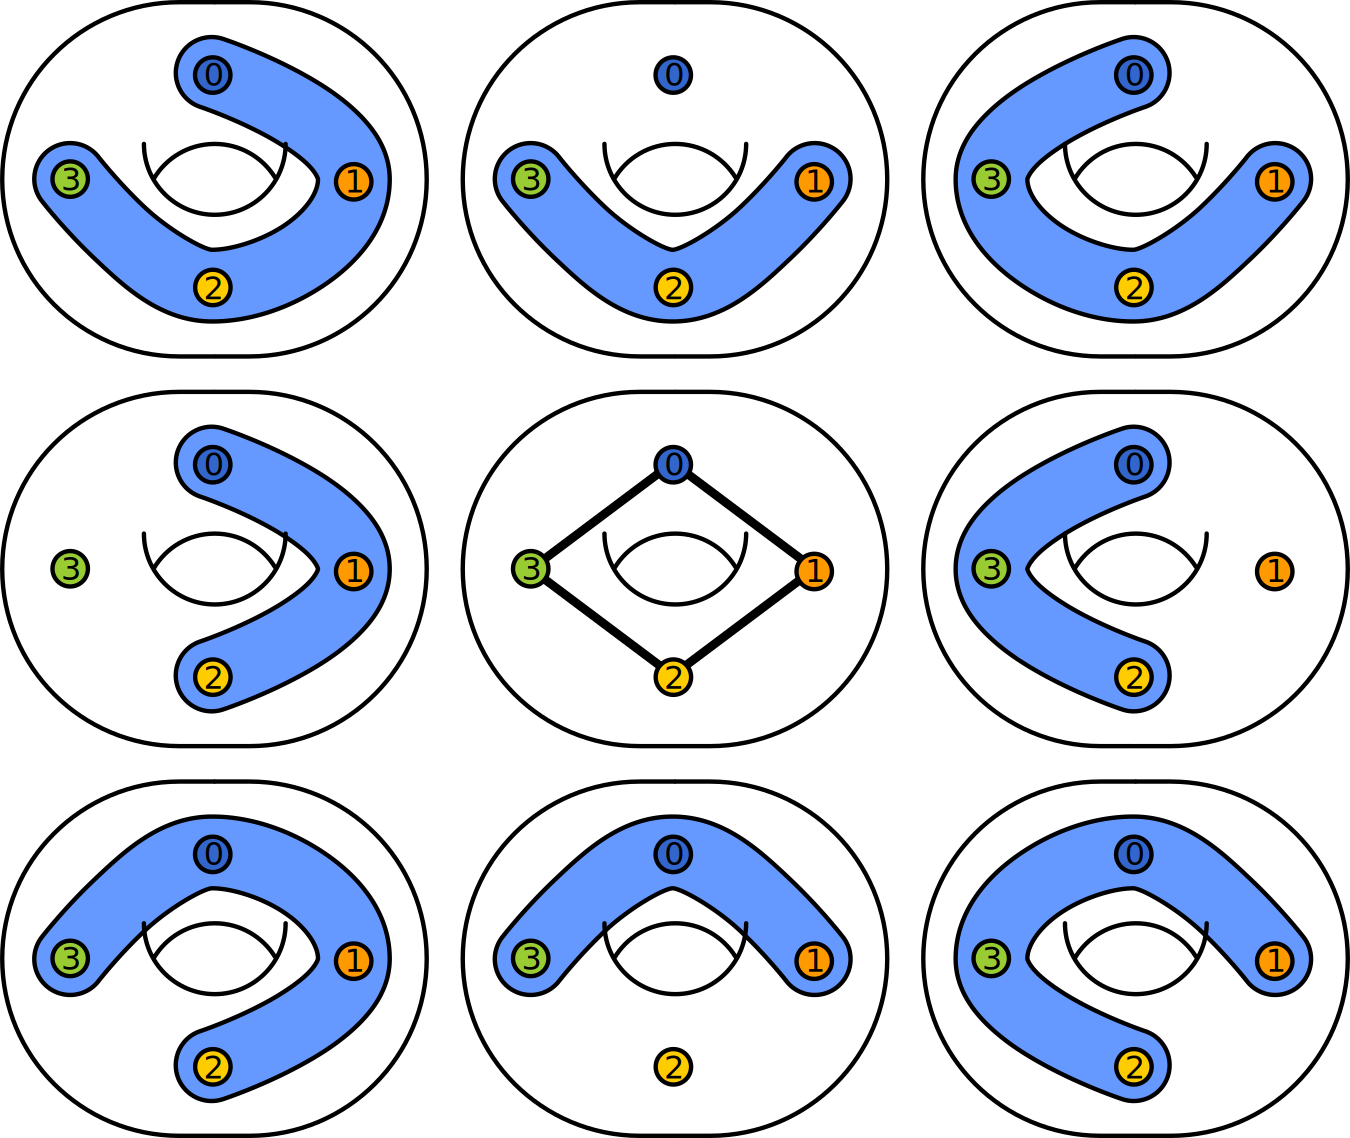
\includegraphics[width=.6\textwidth]{figures/standardoctagon.pdf}
  \caption{The standard octagon in $\css S_{1,4}$. The octagon consists of
  the 8 punctured disks around the outside. Representing arcs are shown in the middle.}
  \label{fig:standardoctagon}
\end{figure}


\begin{conjecture}
 Any octagon of $\css S_{1,4}$ that has the point configuration
 $(p_0,p_1,p_2,p_3)$ is homeomorphic to the standard octagon
 shown in Figure \ref{fig:standardoctagon}.
 \label{conjoct}
\end{conjecture}

\begin{lemma}
  If Conjecture \ref{conjoct} is true then automorphisms of $\css S_{1,4}$
  preserve the standard octagons.
  \label{lemma:stdoctpres}
\end{lemma}

\begin{proof}
  Assume that Conjecture \ref{conjoct} is true.
  We will show that an octagon has point configuration $(p_0,p_1,p_2,p_3)$
  if and only if the pairs of 4-punctured disks at distance four
  have infinitely many
  distinct length 4 paths in $\css S_{1,4}$, and
  the pairs of 3-punctured disks at distance four
  have finitely many
  distinct length 4 paths in $\css S_{1,4}$

  Let $\mathcal O =(x_i,y_i)_{i \in 4}$ be a standard octagon.
  In light of Conjecture \ref{conjoct} there is an arc $\alpha$ between the
  two punctures $P(x_i)\cap P(x_{i+1})$ that is in $y_{i-1}, x_i, y_i, x_{i+1}, y_{i+1}$.
  Then the half twist $T_\alpha$ fixes $y_{i-1}, x_i, y_i, x_{i+1}, y_{i+1}$, but
  does not fix $x_{i+2}, y_{i+2}, x_{i-1}$ so that
  $$
  y_{i-1}, T^n_\alpha x_i, T^n_\alpha y_i, T^n_\alpha x_{i+1}, y_{i+1}
  $$
  is a distinct length 4 path of $\css S_{1,4}$ for every $n$.

  We further claim that there are finitely many paths of length 4 between $x_0$ and $x_2$, and similarly between $x_1$ and $x_3$.
  Let $$x_0 \to y_{0,n} \to x_{1,n} \to y_{1,n} \to x_2$$ be a distinct path in $\css S_{1,4}$
  for every $n \in \Z$.
  Then there are two integers $n,n'$ such that $P(x_{1,n})=P(x_{1,n'})$,
  but then these paths would give an octagon with point configuration
  $(p_0,p_1,p_2,p_1)$ or $(p_0,p_3,p_2,p_3)$ which would contradict Lemma \ref{lemma:ptconfig}.
  It must be that there are exactly two paths of length 4 between $x_0$ and $x_2$ in $\css S_{1,4}$.
  Similarly there are exactly two paths of length 4 between $x_0$ and $x_2$ in $\css S_{1,4}$.

  Suppose that $\mathcal O =(x_i,y_i)_{i \in 4}$ is an octagon with point configuration
  $(p_0,p_0,p_1,p_1)$.
  Assume to the contrary that
  there are infinitely many distinct paths
  $$
  y_3 \to x_{0,n} \to y_{0,n} \to x_{0,n} \to y_1
  $$
  for $n \in \Z$.
  Then since
  $$
  y_3\to x_{0,n}\to y_{0,n} \to x_{1,n} \to y_1 \to x_2 \to y_2 \to x_3
  $$
  is an octagon so by Lemma
  \ref{lemma:ptconfig}, it must be that
  the point configurations are equal $P(x_{0,n})=P(x_{1,n})$.
  But then since there are infinitely many length four paths $y_3$ to $y_1$,
  so there must be two integers $n,n'$ such that $P(x_{0,n})=P(x_{0,n'})$.
  But then those paths together give an octagon with point configuration
  $(p_0,p_0,p_0,p_0)$ or $(p_1,p_1,p_1,p_1)$ in contradiction to Lemma \ref{lemma:ptconfig}.

  Suppose that $\mathcal O =(x_i,y_i)_{i \in 4}$ is an octagon with point configuration
  $(p_0,p_1,p_0,p_1)$.
  Let $\alpha_i$ be an arc of $x_i$ between $p_2$ and $p_3$.
  Then the loop $\alpha_i\cev \alpha_j$, for the reversed arc $\cev \alpha$, is contained in a 4-curve
  so it is trivial in the unpunctured torus.
  The $x_2$ is determined by one additional arc $\alpha'$ from $p_1$ to $p_2$,
  so that $x_0$ and $x_2$ do not fill the torus.
  There must be a nonseparating loop $\beta$ of the torus based at $p_0$
  which is disjoint from both.
  Let $\psi_\beta$ be the point pushing map pushing $p_0$ along $\beta$.
  The loop $\beta$ intersects the four curves, so
  Then
  $$x_0 \to \psi^n_\beta y_0 \to \psi^n_\beta x_1 \to \psi^n_\beta y_1 \to  x_2$$
  for all $n\in \Z$ gives infinitely many distinct length 4 paths from $x_0$ to $x_2$
  in $\css S_{1,4}$.
\end{proof}

\begin{definition}
  Let $z$ be a 2-punctured disk.
  Define the octagon sharing pair graph $\mathcal {P}^o_z$
  to be the graph defined as follows.
  The vertices of $\mathcal {P}^o_z$  are sharing pairs for $z$ in $\css S_{1,4}$.
  Define two sharing pairs for $z$ to be adjacent in $\mathcal {P}^o_z$ if
  they are contained in two standard octagons $\mathcal O, \mathcal O'$ of $\css S_{1,4}$
  such that the subgraph $\mathcal O \cap \mathcal O'$ is two edges incident at a 4-punctured disk.
\end{definition}

\begin{lemma}
The sharing pair graph  $\mathcal {P}^o_z$ is connected.
\label{lemma:shareoctconnect}
\end{lemma}

\begin{proof}
  We appeal to Putman's Lemma \ref{lemma:putman}.
  Observe that any standard octagon $(x_i,y_i)_{i \in 4}$ can be uniquely
  represented by disjoint arcs $(a_i)_{i \in 4}$ with $a_i$
  in $x_i$ and $x_{i+1}$
  from puncture $p_{i+2}$ to $p_{i+3}$ for $i \in \Z/4$.
  Let two sharing pairs $\{x_0,x_1\}$ and $\{x'_0,x'_1\}$ be adjacent in $\mathcal P^o_z$.
  Then without loss of generality
    $x_0=x_0'$ and there are two octagons $(x_i,y_i)_{i \in 4}$ and $(x'_i,y'_i)_{i \in 4}$
  with representing arcs $(a_i)_{i \in 4}$ and $(a'_i)_{i \in 4}$ respectively
  such that $a_i=a_i'$ for $i=3,0,1$ and  $z$ is a regular neighborhood of $a_0$.

  Fix  a sharing pair $\{x_0,x_1\}$ and let $(a_i)_{i \in 4}$ be the arcs representing an octagon that contains $x_0$ and $x_1$.
  The pure mapping class subgroup fixing the 2-punctured disk $z$
  acts transitively on sharing pairs.
  By Putman's Lemma it suffices to see that
  there is a generating set $H$ for that we can move from $\{x_0,x_1\}$ to $\{hx_0,hx_1\}$
  in $\mathcal P_z$.
  Let $(\alpha_i)_{i \in 4}$ be the disjoint  nonseparating curves such that $\alpha_i$ geometric intersection $1$ with $a_i$. Let $\beta$ be the nonseparating curve disjoint from every $a_i$.
  Let $\gamma$ be the separating curve that the bounds the regular neighborhood of $a_0a_1$.
  Take as a generating pure mapping class subgroup fixing the 2-punctured disk $z$
  the Dehn twists $H=\{T_{\alpha_1},T_{\alpha_2}, T_{\alpha_3}, T_{\beta}, T_\gamma \}$.
  But since each generated fixes either $a_3$ or $a_1$,
  we have that $\{x_0,x_1\}$ is adjacent to $\{hx_0,hx_1\}$ in $\mathcal P^o_z$ for all $h \in H$.
\end{proof}

\begin{proposition}
  If Conjecture \ref{conjoct} is true then
  the natural map $\mcg^\pm S_{1,4} \to \css S_{1,4}$
  is an isomorphism.
\end{proposition}

\begin{proof}
  Assume that Conjecture \ref{conjoct} is true.
  Extend $\phi \in \aaut \css S_{1,4}$ to $\hat \phi \in \aaut \csep S_{1,4}$
  and apply Theorem \ref{thm:sepcurvecomplex}.
  We need only define $\hat \phi$ on 2-punctured disks.

  If $z$ is a two punctured disk let $\{x_0,x_1\}$ be a sharing pair for $z$.
  Choose a standard octagon $\mathcal O$ containing $\{x_0,x_1\}$ as distance 2 3-punctured disks.
  Then by Lemma \ref{lemma:stdoctpres} $\phi(\mathcal O)$ is a standard octagon
  and by Lemma \ref{thm:csstype} $\phi(x_0)$ and $\phi(x_1)$ are 3-punctured disks.
  So $\{\phi(x_0),\phi(x_1)\}$ must also be a sharing pair and we define
  $\hat \phi (z)$ as the 2-punctured disk shared by $\{\phi(x_0),\phi(x_1)\}$.

  It remains only to see that $\hat \phi (z)$ is well defined.
  Suppose that $\{x'_0,x'_1\}$ is another sharing pair sharing $z$.
  By Lemma
  \ref{lemma:shareoctconnect}
  there is sequence of standard octagons $(\mathcal O)_{i =1}^\ell$ with $\{x_0,x_1\}$
  in $\mathcal O_1$ and $\{x'_0,x'_1\}$ in $\mathcal O_\ell$
  such that the subgraph $\mathcal O_i \cap \mathcal O'_{i+1}$ is two edges of $\css S_{1,4}$
  incident at a 4-punctured disk. That is $\mathcal O_i \cap \mathcal O'_{i+1}$
  have in common 3-punctured disks  $x_{0,i}$ and $x_{1,i}$
  and a 4-punctured disk $y_{i}$ adjacent to them in $\css S_{1,4}$,
  and $\{x_{0,i},x_{0,i+1}\}$
  is a sharing pair for $z$ for all $i$.
  But then $\{\phi(x_{0,i}),\phi(x_{0,i+1})\}$ are 3-punctured disks in the sequence of
  standard octagons $(\mathcal O)_{i =1}^\ell$
   $\{\phi(x_{0,i}),\phi(x_{0,i+1})\}$  and  $\{\phi(x_{0,i+1}),\phi(x_{0,i+2})\}$
  sharing pairs for the same 2-punctured disk.
  So $\hat \phi$ is well defined.
\end{proof}

\section{Computational Evidence}
\label{sect:compute}

In this section we examine computational evidence for Conjecture
\ref{conjoct}, which says that any octagon of $\css S_{1,4}$
with a point configuration that is a permutation of
$(p_0,p_1,p_2,p_3)$ is homeomorphic to the standard octagon shown in
\ref{fig:standardoctagon}.

Computations in the curve complex can be performed by representing curves
by their intersection numbers with the arcs of a triangulation of $S_{1,4}$.
We take as our triangulation
 $$
 \begin{tikzcd}
   p_0 \arrow{r}{e_0} & p_1 \arrow{r}{e_3} & p_2 \arrow{r}{e_6} & p_3 \arrow{r}{e_9} & p_0\\
   p_0 \arrow{r}{e_0} \arrow{u}{e_1} & p_1 \arrow{ul}{e_2} \arrow{r}{e_3} \arrow{u}{e_4} & p_2 \arrow{ul}{e_5} \arrow{r}{e_6} \arrow{u}{e_7} & p_3 \arrow{ul}{e_8} \arrow{r}{e_9}  \arrow{u}{e_{10}} & p_0 \arrow{ul}{e_{11}} \arrow{u}{e_1}
 \end{tikzcd}
 $$
 \begin{figure}[h!]
   \centering
   \includegraphics[width=.4\textwidth]{figures/s14compute.pdf}
   \caption{A traingulation of the surface $S_{1,4}$.}
   \label{fig:s14compute}
 \end{figure}
with oriented edges $E=\{e_j\}_{j \in {12}}$.
With this convention any multicurve $x$ is uniquely represented by a tuple in $\Z_{\leq 0}^E$ giving the geometric intersection number $|i|(e_j,x)$.
We refer the reader to \cite{Schaefer2002} for details on these \emph{normal coordinates}.
Normal coordinates
uniquely
determine a number of line segments at each angle of each triangle,
so that any tuple $\Z_{\leq 0}^E$ is a multicurve if and only if it satisfies a triangle inequality for each triangle:
$$
|i|(e_j,x) \leq |i|(e_k,x) + |i|(e_\ell,x)
$$
if $e_j,e_k,e_\ell$ form a triangle and $x$ a multicurve.

From the normal coordinates of a surface we can also compute a nonunique representation
of the curve as a cyclically reduced word
$w(x)$ on the alphabet $E=\{e_j\}_{j \in {12}}$ by choosing a parametrization of $x$ and listing the
edges in the order that they are crossed.
In these coordinates the Dehn twist $T_y(x)$ of $x$ about $y$ is easy to compute
essentially by replacing subwords of $x$ crossing $y$ with an appropriate $w(y)$,
and fast algorithms are known
\cite{fastdehn}.
Hamidi-Tehrani \cite{MR2695693} comptues geometric intersection number $|i|(x,y)$ by
showing that
$$|i|(T^{n+1}_y x ,e_j)-|i|(T^n_y x ,e_j) =  |i|( x ,y)|i|( y ,e_j)$$
for sufficiently large $n$.

Large finite subgraphs of $\css S_{1,4}$ are made easier to compute by the fact that the mapping class group acts transitively on the
edges of  $\css S_{1,4}$.
We have computed a subgraph $\css S_{1,4}$
by iteratively applying a generating set
to the edge shown in \ref{fig:s14edge}.
This is vastly more efficient than computing intersections between known curves to look for disjoint curves,
as the curve complex is $\delta$ hyperblic
so that finite subgraphs $\mathcal C$ of $\css S_{1,4}$
are sparse.

\begin{figure}[h!]
  \centering
  \includegraphics[width=\textwidth]{figures/oct/oneedge.pdf}
  \caption{The curves (1,0,1,0,2,2,0,2,2,1,2,1) and (0,2,2,0,2,2,0,2,2,2,2,2) are disjoint so span an edge of $\css S_{1,4}$.}
  \label{fig:s14edge}
\end{figure}



\begin{figure}[h!]
  \centering
  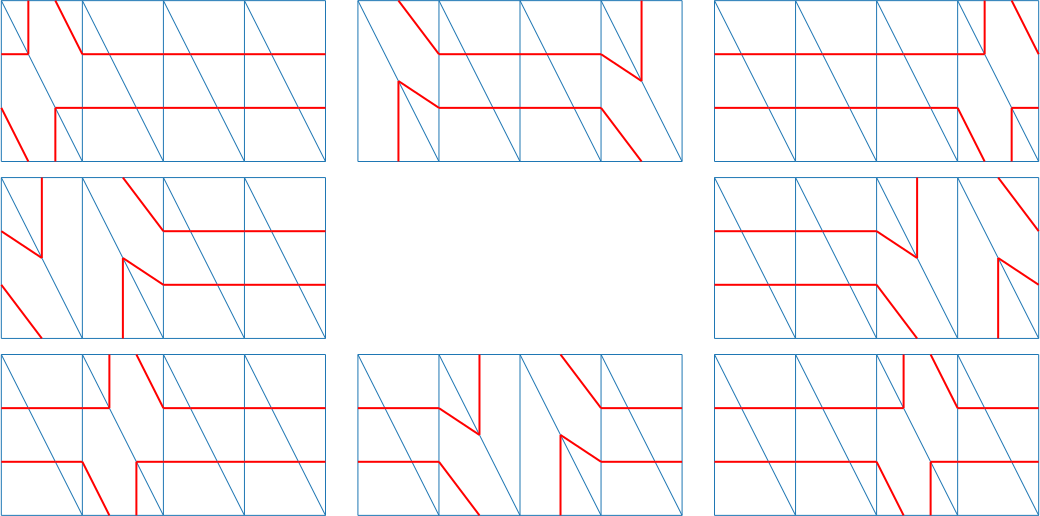
\includegraphics[width=\textwidth]{figures/oct/octstandard1.pdf}
  \caption{The standard octagon represented in normal coordinates.}
  \label{fig:0123oct}
\end{figure}
\begin{figure}[h!]
  \centering
  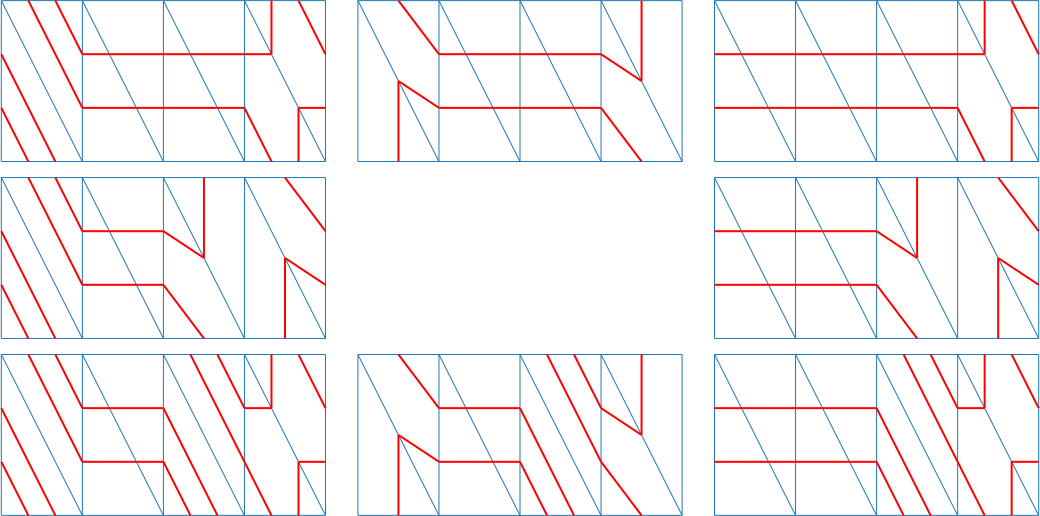
\includegraphics[width=\textwidth]{figures/oct/oct0303.pdf}
  \caption{An octagon with point configuration $(p_0,p_3,p_0,p_3)$ represented in normal coordinates.  }
  \label{fig:0303oct}
\end{figure}
\begin{figure}[h!]
  \centering
  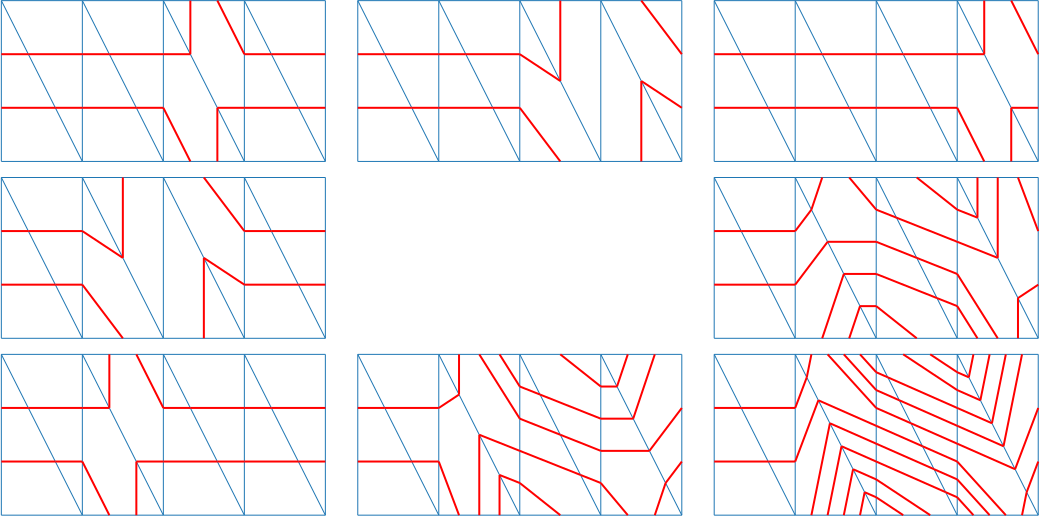
\includegraphics[width=\textwidth]{figures/oct/oct3322.pdf}
  \caption{An octagon with point configuration $(p_3,p_3,p_2,p_2)$ represented in normal coordinates.
  Note the top-left three curves and the bottom-right
  three curves differ by the Dehn twist $T^2_{e_6}$.}
  \label{fig:3322oct}
\end{figure}

Using this we have examined a subgraph $\mathcal C$ of $\css S_{1,4}$
with 105278 edges.
Using standard graph algorithms
we compute
5255 octagons based
at the curve (1,0,1,0,2,2,0,2,2,1,2,1).
Of these 918 octagons have point configurations given by permutations of $(p_0,p_1,p_2,p_3)$.
By computing the $\binom 8 2$ pairwise intersections of the 8 curves, we can verify that these are indeed homeomorphic to
standard octagons, in support of Conjecture \ref{conjoct}.

% 5255 octagons
% 918
% The graph
% $\mathcal C$
% 918 octagons
% (1,0,1,0,2,2,0,2,2,1,2,1)
%
%
%
%
% Also write as crossing sequence, cyclic reduced word in $T^{\pm}$
%
% Computing dehn twists
%
% possible in polynomial time
%
% simplify  $T_\alpha(\beta)$ computation by a choice
% of end for every edge so that $\alpha$ always passes through the end
% and $\beta$ always passes through the middle
%
% Hyperbolicity constant of the curve graph
% Hyperbolicity constant of the strongly separating curve complex
%
% Github
%
% 51516 Three
% 71817 Fourin
% 105278 Pairs of disjoint curves
% Edgelimit 100000
% 100000 edges in G
% 115249 nodes in G
% considering 3655 possible x2
% considering 4194 possible x2
% 5255 octagons found based at (0, 4) (1, 0, 1, 0, 2, 2, 0, 2, 2, 1, 2, 1)
%


% \section{  JibJab Nonsense }
%
% \subsubsection{$S_{1,5}$}
%
% \begin{lemma}
%   ??Curve types are preserved
%   There's hexagons inside a 5 curve.
%   There's no hexagons outside a 3 curve since there's no hexagons in $S_1,4$?
% \end{lemma}
%
% \begin{definition}
% 3-disk sharing pair is $x_0,x_1$ such that there is
% $$
% \begin{tikzcd}[column sep={1cm,between origins}, row sep={1.732050808cm,between origins},every arrow/.append style={dash}]
%     & x_0 \arrow[rr] \arrow[rd] \arrow[ld] && y_0 \arrow[rd] \arrow[ld]  &  \\
%     y_2 \arrow[rd]\arrow[rr]&  & z \arrow[rr] &  & x_1 \\
%     & x_2 \arrow[rr] \arrow[ur] && y_1 \arrow[ru]\arrow[lu] &
% \end{tikzcd}
% $$
% so that $z$ is a 5-disk, $y_i$ are 4-disks, $x_i$ is a 3-disk
% \end{definition}
%
% \begin{lemma}
%   The complex of 3 and 4-disks in an annulus
%   has no cycles smaller than an octagon.
% \end{lemma}
%
% \begin{lemma}
%   Suppose hexagon $(x_i,y_i)_{i \in \Z/3}$ as above.
%   If $y_0$ and $y_1$ have geometric intersection 2,
%   and $p_0, p_1$ are in $y_0 \cap y_1 \cap y_2$,
%   then there is a unique 2-curve shared by $y_0,y_1,y_2$.
% \end{lemma}
% \begin{proof}
%   Observe if there is a 2-disk, it has to be unique as
%   if there are a pair of 2-disk shared by all $y_i$,
%   then that would give a 3-disk shared by all $y_i$.
%
%   Assume to the contrary there's no path
%    $p_0$ and $p_1$ all three $y_i$.
%    There there are arcs $\alpha$ and $\beta$
%    from $p_0$ to $p_1$ with $\alpha \subset x_0\subset y_0$
%    and $\beta \subset x_2 \subset y_1$.
%    Then $\alpha\beta^{-1}$ is a nontrivial loop that must be contained in the disk $y_2$.
%    So
%    Consider the projections of $\alpha$ and $\beta$ in the bigon $y_0 \cap y_1$.
%    $\alpha$ has arcs from $p_0,p_1$ to the $y_0$-edge of the bigon,
%    similarly
%    $\beta$ has arcs from $p_0,p_1$ to the $y_1$-edge of the bigon,
%    so that these four arcs form a band across the bigon.
%   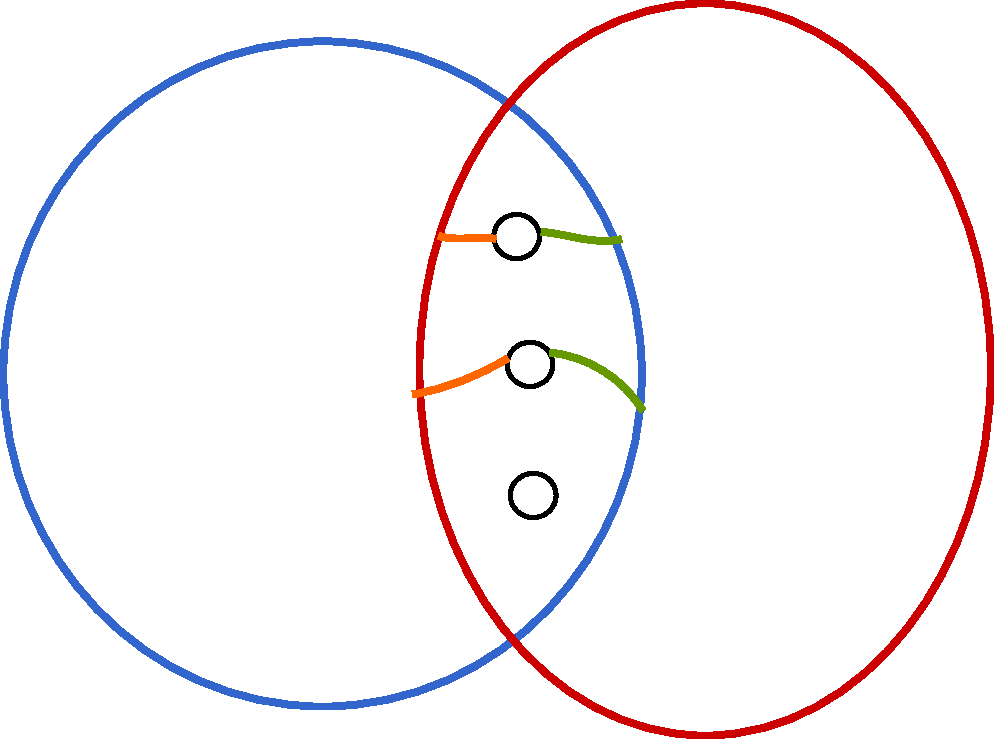
\includegraphics[width=.2\textwidth]{figures/2curveinbigon.pdf}
%   No arc of $\alpha,\beta$ can disconnect the band, so the band
%   there must contain a path $p_0$ to $p_1$ which is in $y_1$.
%   % \includegraphics[width=.5\textwidth]{figures/outofx0.pdf}
%
% \end{proof}
%
%
% \begin{lemma}
% A 3-disk sharing pair uniquely determines a 3-disk.
% \end{lemma}
% \begin{proof}
%   We are working in the 3 \& 4-disk complex of a 5-disk.
%   Consider the possible distribution of the marked points
%   $p_0,\ldots,p_4$
%   in the 5-disk.
%   If there is a point that is in none of the 4-disks $y_i$,
%   then we would have a hexagon in the 3 \& 4-disk complex of an
%   annulus.
%   So up to relabeling
%   $p_4 \not \in y_0$ and $p_3 \not \in y_1$ and there are
%   three cases for 4-disk point configuration
%
%   Case 0: $p_2 \not \in y_2$
%
%   Case 1: $p_4 \not \in y_2$ and $p_2 \not \in x_0$2
%
%
%
%   Claim that $\partial y_0$ and $\partial y_1$ have
%   geometric intersection 2.
%   The 3-disk $x_1$ is contained in both $y_0$ and $y_1$.
%   So there is only one possible projection for $y_1$ into $y_0$ bands.
%   The idea is supposed to be find two arcs in $y_2$
%   that you assume are disjoint but the bands get in the way
%   Now $p_0,p_3 \in x_0 \subset y_0 \cap y_2$
%   and $p_1,p_4 \in x_2 \subset y_1 \cap y_2$.
%
%
%   Case 2: $p_4 \not \in y_2$ and $p_3 \not \in x_0$
%
%   Claim that $\partial y_0$ and $\partial y_1$ have
%   geometric intersection 2.
%   The 3-disk $x_1$ is contained in both $y_0$ and $y_1$.
%   So there is only one possible projection for $y_1$ into $y_0$ bands,
%   which separate $p_3$ from $x_1$ in $y_0$.
%   Now  $p_0,p_1,p_2 \in x_2 \subset y_1\cap y_2$ so there must be an arc $\alpha$
%   from $p_0$ to $p_1$ contained in $x_2$ but not in $x_1$ so it must
%   pass through the bands.
%   Similarly $p_0,p_1,p_2 \in x_0 \subset y_2 \cap y_0$
%   so there must be an arc $\beta$ from $p_0$ to $p_1$ contained in $x_0$
%   but not in $x_1$, so it must cross the bands.
%   But then $\beta$ and $\alpha$ form a bigon around $p_3$ so that $p_3$ must be in $x_1$, a contradiction.
%
%   Now $p_0$ and $p_1$
%   arc $\alpha$ from $p_0$ to $p_1$
%   arc $\beta$ from $p_0$ to $p_1$
%
%
%   The idea is supposed to be find two arcs in $y_2$
%   that you assume are disjoint but the bands get in the way
%   Now $p_0,p_3 \in x_0 \subset y_0 \cap y_2$
%   and $p_1,p_4 \in x_2 \subset y_1 \cap y_2$.
%
%
%
%   Then you're supposed to assume that the $p_0\to p_1$
%   arcs in $x_2$ and $x_0$ are not in $x_1$ so they have to be distinct and you force
%   them to bound a disk that has to be in $y_2$ and show that defines the 4-curve and
%   then its not the one you want?
%
% \end{proof}
%
%
% \subsection{ Octagonal Sharing Pairs?}
%
% Observe that $C^{ss}(S_1,4)$ is a bipartite graph consisting of
% 3-disks and 4-disks.
%
% Consider a $2n$-cycle $(x_i,y_i)_{i \in 2n}$ in $C^{ss}(S_{1,4})$
% with $x_i$ a 3-disk and $y_i$ a 4-disk.\\
%
%
%
%
% % \emph{Claim} In an octagon $x_i$ and $x_{i+1}$,
% %  there is a unique 2-disk in both $x_i$ and $x_{i+1}$.\\
%
% \emph{Def}
% Let $A_{p,q}$
% be the set of classes of arcs from point $p$
% to point $q$ considered up to homotopy relative to $P$.
% By forgetting all the points but $p$ and $q$
% we may also consider the arcs $A_{p,q}$
% up to homotopy relative to ${p,q}$.
% Observe that if $a, a' \in A_{p,q}$
% are arcs contained in a common 4-disk then $a$ and $a'$ are homotopic relative to $\{p,q\}$.
%
% \vspace{1cm}
%
% \emph{Claim} Suppose that $x_0$ and $x_2$ are distance four
% 3-disks in an octagon.
% Then $x_0$ and $x_2$ contain the same points
% if and only if there more than 2 length 4 paths from $x_0$ to $x_2$.\\
% \\
% Suppose that there are at least 3 paths from $x_0$ to $x_2$,
% each of which pass through a distinct 3-disk, say $x_1$, $x_2$, $x_3$.
% If $x_1$, $x_2$, $x_3$ all contain distinct sets of marked points,
% then by the possible point configurations
% described by Lemma , there are not possible choice for the
% marked points contained in $x_0$ and $x_2$.
% If two of  $x_1$, $x_2$, $x_3$ contain the same points.
% But then by the possible point configurations
% described by Lemma , the $x_0$ and $x_2$ must also contain the same points.
%
% Suppose $x_0$ and $x_2$ contain the same points, say $p_1,p_2,p_3$.
% Then by the Lemma
% it must be that $x_1$ and $x_3$ contain the same points,
% say $p_0,p_1,p_2$.
% Suppose that there is a nonseparating curve $\alpha$ based at $p_0$
% and disjoint from $x_0$ and $x_2$.
% Let $$x_0,y,x,y',x_2$$ be a length 4 path.
% Since $p_0 \in y,x,y'$
% we have that
% $$x_0 \to T^k_\alpha y \to T^k_\alpha x \to T^k_\alpha y'\to x_2$$
% gives infinitely many paths of length 4.
%
% If there is no nonseparating curve then $p_0$ is in 2n-gon. Connect p0 to all the corners!
%
%
%
%
%
%  \emph{Claim}
%  Up to homeomorphism
%  there is only one
%  type of octagon with $p(x_i) =\{p_j\}_{j \neq i}$.\\
%  \\
%
%
%
% 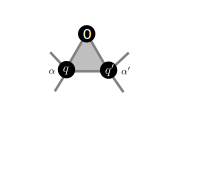
\includegraphics[width=.5\textwidth]{figures/nobigonsrotycase.pdf}
%
% Consider the two 3-disks
% $x_0$ and $x_2$. Observe that $x_0$ and $x_2$ cannot be contained in
% a common 4-disk, or else $x_0,x_1,x_2$ would all be contained in a common
% 4-disk which would force $y_0=y_1$ by Lemma .
%
% Assume to the contrary that $x_0$ and $x_2$
% contain a common arc $a_{13} \in A_{p_1,p_3}$.
% Consider arcs $a^{(0)}_{12} \in A_{p_1,p_2}$ in $x_0$
% and $a^{(2)}_{10} \in A_{p_1,p_0}$ in $x_2$
% which cannot be contained in a common 4-disk,
% since otherwise a regular neighborhood of $a_{12} \cup a^{(0)}_{13} \cup a^{(2)}_{01}$
% is a 4-disk containing $x_0$ and $x_2$.
% Then $x_3$ contains arcs
% $a^{(3)}_{12} \in A_{p_1,p_2}$,
% which must be homotopic to $a^{(0)}_{12}$ relative to $p_1,p_2$,
% and
% $a^{(3)}_{10} \in A_{p_1,p_0}$,
% which must be homotopic to $a^{(2)}_{10}$ relative to $p_1,p_0$.
% But then $a^{(3)}_{12}$ and $a^{(3)}_{10}$
% cannot be contained in a common 4-disk, and yet are contained in $x_3$, a contradiction.
%
% Let $a^{(i)}_{i+1,i+2} \in A_{p_{i+1}, p_{i+2}}$ for $i \in 4$
% be an arc in $x_{i}$.
% Then we have a
% loop $a=a^{(0)}_{12}a^{(1)}_{23}a^{(2)}_{30}a^{(3)}_{01}$
% of $S_1$.
% We may assume any self-intersections of $a$ occur
% transversely at points not in $P$.
%
% Assume to the contrary that $a$ is nullhomotopic in $S_1$.
% % Then there is a non-embedded disk $D\subset S_1$
% % with $\partial D = a$ which cannot be contained in a 4-disk of $S_{1,4}$.
% So $a$ must be a non-simple separating curve in the torus.
% There must be a point $p \in P$
% such that $a$ is not nullhomotopic relative to $\{p\}$.
% Relabel $P$ so that $a$ is not nullhomotopic relative to $\{p_0\}$.
% So $a$ forms an innermost bigon $b$ with itself with $p_0$ on one side.
% Let $q,q' \in a$ be the vertices of the bigon.
% \includegraphics[width=.5\textwidth]{figures/abigon.pdf}
% The image of $a-(b-q)$ must contain a simple closed curve $\alpha$ based
% at $q$,
% and
% $a-(b-q')$ contains a simple closed curve $\alpha'$ based
% at $q'$.
% Since $a^{(i)}$ and $a^{(i+1)}$ must be contained in a common 4-disk,
% their union cannot contain loops of the torus.
% So both $\alpha$ and $\alpha'\subset a$
% must have at least 2 points of $P -\{0\}$, but
% they do not intersect at $P$, a contradiction.
%
% Assume to the contrary that $a$ is not homotopic in $S_1$
% to a simple closed curve of $S_1$.
% Let $q$ be a self-intersection of $a$
% and let $\alpha$ and $\alpha' \subset a$ be two nontrivial loops of $S_1$
% sharing no common subarcs.
% Then $\alpha$ and $\alpha'$ must each contain two points of $P$.
% Say $\alpha$ contains $p_0$ and $p_1$ while $\alpha'$ contains $p_2$ and $p_3$.
% So $a^{(0)}_{12}$ and $a^{(2)}_{30}$
% must intersect at $q$.
% Observe $x_1$ must contain an arc $a^{(1)}_{30} \in A_{p_3p_0}$
% homotopic to $a^{(2)}_{30}$ relative $\{p_3p_0\}$
% and disjoint from $a^{(1)}_{23} - \{p_3\}$.
% Then $a^{(2)}_{30}$ and $a^{(1)}_{30}$ cannot be homotopic relative to $P$,
% as if $a^{(1)}_{30}$ intersects $a^{(0)}_{12}$
% the 4-disk $y_0$ would contain $\alpha'$.
% Then $a^{(1)}_{23}$ must
% link with $a^{(3)}_{01}$.
% But then $a^{(3)}_{01}$ is homotopic relative $\{p_0,p_1\}$
% to a curve
% $a^{(2)}_{01} \in A_{p_0p_1}$ in $x_2$ which must link with $a^{(1)}_{23}$.
% But then $y_1 \supset x_1\cup x_2$ contains a nontrivial loop of the torus.
% It must be that $a$ is a homotopic in $S_1$ relative
% $\varnothing$ to a simple closed curve of $S_1$.
%
% Let $b$ be the simple closed curve obtained from $a$
% by homotoping the arcs $a^{(i-1)}_{i,i+1}$ relative ${p_i,p_{i+1}}$.
% We may assume that $a^{(3)}_{01}=b^{(3)}_{01}$.
% \includegraphics[width=.5\textwidth]{figures/stayinannulus.pdf}
% Assume to the contrary that
% $a^(0)_{12}$
% is not supported on the annulus $N(b)$.
% Then let $D$ be an innermost bigon formed by $a^{(0)}_{12}$ and
% $b^{(3)}_{12}$, which must contain
% a point of $P-\{p_1,p_2\}$.
%
% If
% $a^{(0)}_{12}$ and
% $a^{(3)}_{01}$ intersect at a point $q \in \partial D$,
% then $a^{(3)}_{01}$ has an arc that cros
%  $a^{(0)}_{12}$
% contains a loop
%
% % Since $p_1,p_2 \in D$ it must be that
% % $a^{(3)}_{01}$ intersects
% % $b^{(0)}_{12}$ an even number of times, including $p_1$,
% % so the interior of the arcs intersect an odd number of times.
% % So the interiors of $a^{(3)}_{01}$ and $a^{(0)}_{12}$
% % intersect an odd number of times. Let $q$ be such an intersection point.
% % Then $a^{(3)}_{01} \cup a^{(0)}_{12}$ contains an arc $b'_{12}$ which cannot
%
%
%
% % Assume to the contrary that $x_0$ and $x_3$ do not contain a common
% % 2-disk.
% % Let $z \subset x_0$ be a 2-disk containing $p_1$ and $p_2$
% % Consider the image of $x_3$ in $S_{1,4}/z$.
% % As  $p_0 \in x_3$ the 3-disk $x_3$ must contain a bigon containing $p_0$
% % with one edge on $\partial z$.
% % It must be that $x_3$ contains a band $b \subset y_3$
% %  winding around $p_0$ to connect $p_1$ and $p_2$.
% % Further $x_3$ must contain a band $b' \subset y_3$ winding around $p_3$ to connect
% % $p_0$ to $p_1,p_2$.
% % As $x_3 \not \subset y_1$ there must be a nonseparating curve $\alpha \subset y_1^c$
% % that intersects $x_3$. Since $\alpha$ is disjoint from $x_0$,
% % it must separate $y_3$ into components containing $p_0$
% % and separately $p_1,p_2,p_3$.
% % This forces the components of $x_3 - \alpha$ to separate $p_1$  from
% % $p_2$
% % from $p_3$.
% % Then there is an arc $a_1 \subset x_1$ from $p_0$ to $p_3$.
% % Since $a_1$ is disjoint from $\alpha$ it has a nontrivial image in $S_{1,4}/y_3$.
% % Consider an arc $a_2 \subset x_2$ from $p_3$ to $p_0$.
% % Since $a_1a_2 \subset y_1$ is trivial in the unpunctured torus,
% % $a_2 \not \subset y_3$ and $a_2$ must have
% % parallel arcs to $a_1$ in $S_{1,4} -y_3$.
% % If $a_2$ is disjoint from $\alpha$, then $x_3 \cup a_2$
% % contains a nontrivial loop in the unpunctured torus, contradicting that $x_3\cup a_2 \subset y_2$.
% % So $a_2$ must intersect $\alpha$.
% % Consider the subarc $a_1' \subset a_1 \cap y_3$
% % from a point $q_0 \in \partial y_3$ to $p_0$.
% % Since $a_2$ intersects $\alpha$ it must intersect $a'_1$.
% % But then $a_1 \cup a_2$ cannot be contained in $y_1$, a contradiction.
% % It must be that $x_0$ and $x_3$ contain a common 2-disk.\\
%
%
% %  \emph{CASE 2}
% %  Suppose
% % $p(x_0)=p(x_2)=\{p_1,p_2,p_3\}$ and $p(x_1)=p(x_3)=\{p_0,p_1,p_2\}$
% %  \\
% %
% % Observe all curves contain the points $p_1$ and $p_2$.
% % Assume to the contrary that $x_0$ and $x_3$ do not contain a
% %
% %
% % COLLAPSE 3-disks to look throw out arcs that aren't contained in adjacent 3-disks.
% % %
% % Consider the image of $x_3$ in $S_{1,4}-x_0$.
% % The 3-disks $x_0$ and $x_3$ must be contained a 4-disk $y_3$ distinct from $y_1$,
% % so $x_3$ contains either a similar band $b'$ such that $b'^c \cap b^c$ contains a bigon containing $p_0$,
% % or $x_3$ contains a bigon containing $p_0$ with one side on $x_0$.
% % Consider the 4-disk $y_2$, which contains $x_2$ and $x_3$.
% % If $y_2$ also contained $x_0$, then $y_2$ would be a 4-disk containing $x_3$ and $x_0$,
% % and we would have $y_2$ homotopic to $y_3$, a contradiction.
% % So $y_2$ must  intersect $x_0$, and in particular
% % we must be able to write $y_2$ as the complement of a regular neighborhood of
% % a pair of intersection 1 nonseparating arcs $\alpha$ and $\beta$
% % with $\alpha$ intersecting $x_0$.
% % % Observe that $\alpha$ is disjoint from $x_2$ and $x_3$
% % So $\alpha$ cuts  $y_0$ into at least two components.
% % Since $x_3$ and $x_0$ contain at least two points in common
% % we may assume $p_1$ and $p_2$ are contained in $x_0$ and $x_3$.
% % Then as $\alpha$ intersects $x_0$ but not $x_2 $in $y_3$, it must be that
% % $p_1$ and $p_2$ are contained in a common component of $x_0 -\alpha$
% % and a different component than $p_3$.
% %
% %
% %
% %
% % Consider what points $x_2$ may contain.
% % Suppose that $p_3 \in x_2$.
% % As $x_2$ must contain $p_1$ or $p_2$,
% % say $p_1 \in x_2$.
% % Then $x_2$ contains an arc $a_2$ from $p_1$ to $p_3$
% % Observe that $a_2\subset x_2 \subset y_2$ is disjoint from $\alpha$.
% % So $S_1 -\alpha$ is an annulus with
% %
% % But $x_1$ contains an arc $a_1$ from $p_3$ to $p_1$
% % which must intersect $\alpha$
% % an odd number of times as $p_3$ and $p_1$
% %  are in separate components of $y_0-\alpha$.
% % So $a_1a_2$ gives a nontrivial nonseparating curve in the torus and
% % contained in $y_1$, contradicting that $y_1$ is a 4-disk.
% %
% % Then $p_0,p_1,p_2 \in x_2$, so the band $b$ intersects $x_2$ since $x_2$ is not contained in $y_1$.
% % But then $x_2$ and $x_1$ cannot be contained in a common 4-disk.\qed
%
%
%
%
%
%
% \noindent \emph{Remark }
% Fix a 2-disk $z$
% A pair ${x,x'}$ of 3-disks containing $z$ are
% a sharing pair for $z$ if they fit into a common octogon.
% Call a triple ${x,x',x''}$ of 3-disks containing $z$
% a sharing triple if every two form a sharing pair.
%
% Make a graph $P_z$ whose vertices are sharing pairs ${x,x'}$
% of $z$ and with two sharing pairs adjacent if
% their union is a sharing triple.
%
% Well-definedness is shown by Putman's Lemma on $P_z$.
% Observe that only two of the generators move the sharing pair
% at all and only distance 1.
%
% 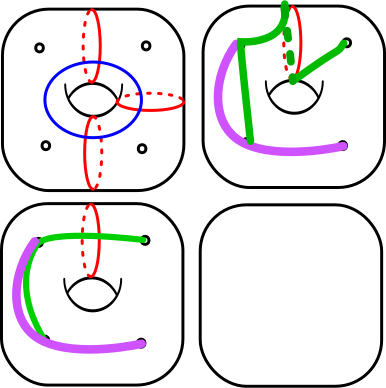
\includegraphics[width=.5\textwidth]{figures/s14.pdf}
